\documentclass{article}
%
% Demo of the mcode package from 
% http://www.mathworks.co.uk/matlabcentral/fileexchange/8015-m-code-latex-package
% Updated 06 Mar 2014
%

% load package with ``framed'' and ``numbered'' option.
\usepackage[framed,numbered,autolinebreaks,useliterate]{mcode}
\usepackage{graphicx}
\usepackage{mathtools}
\usepackage{enumitem}
\usepackage{amsfonts}
\usepackage{amsmath, amsthm, amssymb, amsfonts}
\usepackage{ upgreek }
\usepackage{ tipa }
\usepackage{bbm}
\usepackage{hyperref}
\usepackage{fancyhdr}
\usepackage{mathrsfs}
\pagestyle{fancy}
\rhead{Evans Chapters 5 - 9}
\lhead{}
\hypersetup{
    colorlinks=true,
    linkcolor=blue,
    filecolor=magenta,      
    urlcolor=cyan,
    pdftitle={Evans PDE},
    bookmarks=true,
    %pdfpagemode=UseOutlines,
}
\DeclarePairedDelimiter{\norm}{\lVert}{\rVert} 
\newtheorem{theorem}{Theorem}
\newtheorem{lemma}[theorem]{Lemma}
\newcommand{\avint}{⨍}
\def\Xint#1{\mathchoice
{\XXint\displaystyle\textstyle{#1}}%
{\XXint\textstyle\scriptstyle{#1}}%
{\XXint\scriptstyle\scriptscriptstyle{#1}}%
{\XXint\scriptscriptstyle\scriptscriptstyle{#1}}%
\!\int}
\def\XXint#1#2#3{{\setbox0=\hbox{$#1{#2#3}{\int}$ }
\vcenter{\hbox{$#2#3$ }}\kern-.6\wd0}}
\def\ddashint{\Xint=}
\def\dashint{\Xint-}

\newtheorem{innercustomgeneric}{\customgenericname}
\providecommand{\customgenericname}{}
\newcommand{\newcustomtheorem}[2]{%
  \newenvironment{#1}[1]
  {%
   \renewcommand\customgenericname{#2}%
   \renewcommand\theinnercustomgeneric{##1}%
   \innercustomgeneric
  }
  {\endinnercustomgeneric}
}

\newcustomtheorem{customthm}{Theorem}
\newcustomtheorem{customlemma}{Lemma}
\newtheorem{thm}[equation]{Theorem}


\usepackage[
backend=apa6,
]{biblatex}

\usepackage{titlesec}
\titleformat{\subsection}[runin]{}{}{}{}[]

\setcounter{secnumdepth}{0}
 
\addbibresource{mybib.bib} %Imports bibliography file

\usepackage[margin=1.5in]{geometry}


% something NOT relevant to the usage of the package.
\usepackage{url}
\setlength{\parindent}{0pt}
\setlength{\parskip}{8pt}
%\pagenumbering{gobble}
\title{\texttt{Solutions to Partial Differential Equations by Lawrence Evans}}
\author{Matthew Kehoe}
% //////////////////////////////////////////////////

\renewenvironment{abstract}
 {\par\noindent\textbf{\abstractname.}\ \ignorespaces}
 {\par\medskip}

\begin{document}
\maketitle
\begin{flushleft}
\begin{abstract}
These are my solutions to selected problems from chapters 5--9 of Partial Differential Equations by Lawrence Evans. Any mistakes in these solutions are my own. I plan to write more solutions in the future. If you would like to speak with me about these solutions (or about anything related to PDEs) then I can be contacted at \href{mailto:mkehoe5@uic.edu}{mkehoe5@uic.edu}.
\end{abstract}
\tableofcontents

\maketitle
\phantomsection
\section{Chapter 5 Solutions}
\phantomsection
\subsection{\textbf{5.10.4}} Assume $n=1$ and $u\in W^{1,p}(0,1)$ for some $1 \le p < \infty$. \begin{enumerate}[label=(\alph*)]
    \item Show that $u$ is equal a.e. to an absolutely continuous function $u'$ (which exists a.e.) belongs to $L^p(0,1)$.
    \item Prove that if $1<p<\infty$, then
    $$|u(x)-u(y)| \le |x-y|^{1-\frac{1}{p}}\left(\int_0^1 |u'|^p\,dt\right)^{1/p}$$
    for a.e. $x,y\in[0,1]$.
\end{enumerate}

We first state a lemma summarizing the relationship between absolutely continuous functions and the fundamental theorem of calculus.
\begin{lemma}A function $U$ on $[a,b]$ is absolutely continuous if and only if 
$$U(x) = U(a)+\int_a^x u(t)\,dt$$
for some integrable function $u$ on $[a,b]$.
\end{lemma}
\begin{proof}
The sufficiency part of the lemma follows directly from the fundamental theorem of calculus. That is, if $u$ is integrable on $[a,b]$, and if $U$ is defined by 
$$U(x):=\int_a^x u(t)\,dt,\quad a\le x \le b,$$
then $U'(x)=u(x)$ for almost every $x$ in $[a,b]$. To prove the necessity part, we let $U$ be an absolutely continuous function on $[a, b]$. Then $U$ is differentiable almost everywhere and $U'$ is integrable on $[a, b]$. Let

$$G(x):= U(a)+\int_a^x U'(t)\,dt, \quad x\in[a,b].$$

By the fundamental theorem of calculus, $G'(x)=U'(x)$ for almost every $x\in[a,b]$. It then follows that $(U-G)'(x)=0$ for almost every $x\in[a,b]$. Therefore, $U-G$ is a constant. But $U(a)=G(a)$. Therefore, $U(x)=G(x)$ for almost every $x\in[a,b].$


For $(a)$, let $[a,b]=[0,1]$ and $v(x)=\int_0^x u'(s)\,ds$. Then $v$ is an absolutely continuous function by Lemma 1 (also see Rudin \cite{10.5555/26851} for a proof). Therefore for any test function $\phi\in C_c^{\infty}(0,1):$
\begin{align*}
\int_0^1\big(v(x)-u(x)\big)\phi'(x)\,dx&=
\int_0^1\int_0^x u'(s)\,ds \,\phi'(x)\,dx- \int_0^1 u(x)\phi'(x)\,dx \\&=
\int_0^1\int_s^1 \phi'(x)\,dx \,u'(s)\,ds - \int_0^1 u(x)\phi'(x)\,dx \\&=
-\int_0^1 \phi(s)u'(s)\,ds + \int_0^1 u'(x)\phi(x)\,dx \\&=
-\int_0^1 \phi(x)u'(x)\,dx + \int_0^1 u'(x)\phi(x)\,dx =0.
\end{align*}
As $\phi$ was chosen arbitrarily, we see that $u$ is equal a.e. to an absolutely continuous function $u'$ as required.
For $(b)$, since $u'$ is in $L^p(0,1)$ we apply Holder's inequality with $q=p/(p-1)$:
\begin{align*}
|u(x)-u(y)| &\le \int_y^x |u'(t)|dt \\&\le \left( \int_y^x dt\right)^{(p-1)/p} \left( \int_y^x |u'|^p dt \right)^{1/p}
\\&\le|x-y|^{1-1/p} \left( \int_0^1 |u'|^p dt \right)^{1/p}.
\end{align*}

\end{proof}
\phantomsection
\subsection{\textbf{5.10.6}}
Assume $U$ is bounded and $U \subset \subset \bigcup_{i=1}^{N} V_i$. Show there exist $C^{\infty}$ functions $\zeta_i$ $(i=1,2,\ldots,N)$ such that
\[
  \begin{cases}
  0 \le \zeta_i \le 1, \quad \operatorname{spt}\text{$\zeta_i \subset V_i$ $(i=1,2,\ldots,N)$} \\
  \sum_{i=1}^N \zeta_i=1 \quad \text{on $U$.}
  \end{cases}
\]
The functions $\{\zeta_i\}_{i=1}^N$ form a \textit{partition of unity}.
\begin{proof}

We first complete problem $5.10.5$. Let $U$ and $V$ be open sets with $V\subset \subset U$. We need to show that there exists a smooth function $\zeta$ such that $\zeta \equiv 1$ on $V$ and $\zeta=0$ near $\partial U$.
\\
\bigskip
As suggested in the hint by Evans, take $V \subset\subset W \subset\subset U$ and let $\varepsilon >0$ be the distance between $V$ and $\partial U$. Then define
$$W:=\Big\{x\in U~: ~d(x,V) < \frac{\varepsilon}{2}\Big\}.$$
By making this distance small enough, we have constructed an open set $W$ which is contained between $U$ and $V$. Let $\tilde{\varepsilon}=\varepsilon/8$. Then
$$\eta_{\tilde{\varepsilon}}(x)=\frac{1}{\tilde{\varepsilon}^n}\eta\left(\frac{x}{\tilde{\varepsilon}}\right)$$
is the required mollifier as suggested in Appendix C of Evans. Define
$$\psi(x):=\eta_{\tilde{\varepsilon}}\ast \chi_W(x),$$
where $\text{spt}(\psi)\subseteq \text{spt}(\eta_{\tilde{\varepsilon}})+\text{spt}(\chi_W)\subset U$ and is therefore a smooth function. Hence
\begin{align*}
    \psi(x) &= \int_{\mathbb R^n} \eta_{\tilde{\varepsilon}}(x-y) \chi_W(y)\,dy \\&=
    \int_{B(x,\tilde{\varepsilon})\cap W} \eta_{\tilde{\varepsilon}}(x-y) \chi_W(y)\,dy \\&= \int_{B(x,\tilde{\varepsilon})\cap W} \eta_{\tilde{\varepsilon}}(x-y)\,dy.
\end{align*}
So if $B(x,\tilde{\varepsilon})\subset W$, we see 
$$\int_{\mathbb R^n} \eta_{\tilde{\varepsilon}}(y)\,dy = \int_{B(0,\tilde{\varepsilon})}\eta_{\tilde{\varepsilon}}(y)\,dy=1,$$
which implies that the support is in $W\cap B(0,\tilde{\varepsilon})$. As $\bar{W}$ is compact, we will cover it and its boundary by open balls. Let 
$$\bar{W}\subset \bigcup_{i=1}^N W_i$$
where $W_i$ denotes an open ball which covers a portion of $W$ and possibly the boundary. Then we may observe that we can use the mollifier $\eta_{\tilde{\varepsilon}_i}$ for every open ball $W_i$ where
$$\psi_i(x):=\eta_{\tilde{\varepsilon}_i}\ast \chi_W(x).$$
By defining
$$\zeta(x):=\sum_{i=1}^N\frac{\psi_i(x)}{\sum_{i=1}^N \psi_i(x)},$$
we observe that for any fixed $x\in U$, only three terms in the sum will be nonzero. As $V \subset\subset W\subset\subset U$, it is clear that $\zeta \equiv 1$ on $V$ and $\zeta=0$ near $\partial U$.

To complete $5.10.6$, we assume $U$ is bounded and $U \subset \subset  \bigcup_{i=1}^N W_i\subset \subset \bigcup_{i=1}^{N} V_i$. So, $U$ has a finite cover $\{V_1,\ldots,V_n\}$ where for every $V_i$, we have a $\psi_i$ as constructed above. The support of $\psi_i$ is contained entirely in $V_i$, $\psi_i\equiv 1$ on $W_i$, and every $\psi_i$ is smooth by definition. Therefore, we define
$$\zeta_i(x):=\frac{\psi_i(x)}{\sum_{i=1}^N \psi_i(x)}$$
where $\sum_i \zeta_i \equiv 1$ by construction and for all $x\in U$, the support of $\zeta_i$ is contained in $V_i$. Also, $\zeta_i$ is smooth because the $\psi_i$ are smooth. Thus, the collection $\{\zeta_i\}_{i=1}^N$ fulfills all of the requirements and is a partition of unity subordinate to the cover $\{V_1,\ldots,V_n\}$.
 
\end{proof}
\phantomsection
\subsection{\textbf{5.10.7}} Assume that $U$ is bounded and there exists a smooth vector field $\alpha$ such that $\alpha \cdot \nu \ge 1$ along $\partial U$, where $\nu$ as usual denotes the outward unit normal. Assume $1\le p < \infty$.
\\
Apply the Gauss-Green Theorem to $\int_{\partial U}|u|^p\alpha\cdot\nu\,dS$, to derive a new proof of the trace inequality
$$\int_{\partial U}|u|^p\,dS\le C\int_U|Du|^p+|u|^p\,dx$$
for all $u\in C^1(\bar{U})$.

\begin{proof}
As $\alpha \cdot \nu \ge 1$ along $\partial U$, we have $|u|^p \le |u|^p \alpha \cdot \nu$. Then
\begin{align*}
    \int_{\partial{U}}|u|^p\,dS &\le \int_{\partial{U}}|u|^p\alpha \cdot \nu\,dS\\&=
    \int_U \nabla\cdot (|u|^p\alpha)\,dx\quad\text{(Gauss$-$Green)}\\&=
    \int_U |u|^p(\nabla\cdot \alpha) + \alpha \cdot \nabla|u|^p\,dx\\&\le
    C\int_U |u|^p + \left|\nabla|u|^p\right|\,dx.
\end{align*}
Therefore, since 
$$\nabla|u|^p=p|u|^{p-1}\text{(sgn $u$)}Du,$$
we have for $p=1$
$$\int_{\partial{U}}|u|\,dS \le C\int_U |u| +|Du|\,dx.$$
On the other hand, if $p>1$ then we apply Young's inequality with $a=|Du|,~ b = |u|^{p-1},~ q=p/(p-1)$ to form
$$\int_U \left|\nabla|u|^p\right|\,dx \le C\int_U p|u|^{p-1}|Du|\,dx\le C\int_U |Du|^p + (p-1)|u|^p\,dx.$$
The constants above are different at every inequality. We may now observe that
\begin{align*}
   \int_{\partial{U}}|u|^p\,dS &\le  C\int_U |u|^p + |Du|^p + (p-1)|u|^p\,dx\\&\le
   C\int_U |u|^p + |Du|^p \,dx,
\end{align*}
as required.

\end{proof}
\phantomsection
\subsection{\textbf{5.10.8}} Let $U$ be bounded, with a $C^1$ boundary. Show that a ``typical" function $u\in L^p(U)$ $(1\le p <\infty)$ does not have a trace on $\partial U$. More precisely, prove that there does not exist a bounded linear operator
$$T:L^p(U)\to L^p(\partial U)$$
such that $Tu=u|_{\partial U}$ whenever $u\in C(\bar{U})\cap L^p(U)$.
\begin{proof} We will construct a counterexample in $L^2(U)$. We need to show that there does not exist a constant $C>0$ such that $\norm{Tu}_{L^2(\partial U)}} \le C\norm{u}_{L^2(U)}}$ for every $u\in L^2(U)$. Let's consider the following  sequence of continuous functions:
$$u_n(x)=\frac{1}{1+n\opernatorname{d}(x,\partial U)},\quad x\in U.$$
Then
$$0\le u_n(x)\le 1,$$
$$\quad u_n(x)=1,~~~x\in \partial U.$$ Therefore, for every $x \in U$,  we see that $u_n(x)\to 0$ pointwise, so by the dominated convergence  theorem
$$\norm{u_n}_{L^2(U)}^2\to 0. $$
However, for every $n$ we have
$$\norm{Tu_n}_{L^2(\partial U)}^2\le C^2 \norm{u_n}_{L^2(U)}^2 \to 0,$$
which implies that the area of the boundary is equal to zero. As $Tu_n=1$ for every $n$ we see that we have arrived at a contradiction. The same analysis works for $L^p(U)$ when $1\le p <\infty$.
\end{proof}
\phantomsection
\subsection{\textbf{5.10.9}} Integrate by parts to prove the interpolation inequality:
$$\norm{Du}_{L^2}\le C \norm{u}_{L^2}^{1/2}\norm{D^2u}_{L^2}^{1/2}$$
for all $u\in C_c^{\infty}(U)$. Assume $U$ is bounded, $\partial U$ is smooth, and prove this inequality if $u\in H^2(U)\cap H_0^1(U).$
\\
(Hint: Take the sequences $\{v_k\}_{k=1}^{\infty}\subset C_c^{\infty}(U)$ converging to $u$ in $H_0^1(U)$ and $\{w_k\}_{k=1}^{\infty}\subset C^{\infty}(\bar{U})$ converging to $u$ in $H^2(U).$)

\begin{proof}
Let $u\in C_c^{\infty}(U)$. Integrating by parts and applying Cauchy–Schwarz in the last inequality forms
\begin{align*}\int_U Du\cdot Du\,dx &\le
C\int_U |u||D^2u|\,dx\quad \\&\le
C\left(\int_U |u|^2\,dx\right)^{1/2}\left(\int_U |D^2u|^2\,dx\right)^{1/2},
\end{align*}
where the boundary term disappears since $u$ has compact support. Taking the square root yields
$$\norm{Du}_{L^2(U)}\le C \norm{u}_{L^2(U)}^{1/2}\norm{D^2u}_{L^2(U)}^{1/2}.$$
Following the hint provided by Evans, since $H_0^1(U)$ is the  closure of $C_0^\infty(U)$ with the norm of $H^1(U)$, we can find a sequence $\{v_k\}_{k=1}^{\infty}$ in $H^1(U)\cap C_c^{\infty}(U)$ converging to $u$ in $H_0^1(U)$. Also, since $\partial U$ is smooth, we can extend $U$ to a set $V$ such that $U \subset \subset V$. Then, by the density of $C_c^{\infty}(V)$, we can find a sequence $\{w_k\}_{k=1}^{\infty}$ in $C^{\infty}(\bar{U})$ converging to $u$ in $H^2(U)$. So, we apply the Gauss$-$Green Theorem and evaluate $Dv_k\cdot Dw_k$ which after one application of Cauchy–Schwarz yields
\begin{align*}\int_U Dv_k\cdot Dw_k\,dx  &\le
C\int_U |v_k||D^2w_k|\,dx\\&\le
C\left(\int_U |v_k|^2\,dx\right)^{1/2}\left(\int_U |D^2w_k|^2\,dx\right)^{1/2},
\end{align*}
where the boundary term once again vanishes because $v_k$ has compact support. As $k\to\infty$,
$$C\left(\int_U |v_k|^2\,dx\right)^{1/2}\left(\int_U |D^2w_k|^2\,dx\right)^{1/2}\to C\left(\int_U |u|^2\,dx\right)^{1/2}\left(\int_U |D^2u|^2\,dx\right)^{1/2},$$
which is equivalent to $C\norm{u}_{L^2(U)}\norm{D^2u}_{L^2(U)}$. To show that the left-hand side converges to $\norm{Du}_{L^2(U)}^2$, we evaluate the difference and once again apply Cauchy–Schwarz
\begin{align*}
    \int_U\left(Dv_k\cdot Dw_k - Du\cdot Du\right)\,dx&=
    \int_U\Big(Dv_k\cdot(Dw_k-Du)+Du\cdot(Dv_k-Du)\Big)\,dx \\&\le
    \int_U |Dv_k|\cdot|Dw_k-Du|+|Du|\cdot|Dv_k-Du|\,dx\\&\le
    \norm{Dv_k}_{L^2(U)}\norm{Dw_k-Du}_{L^2(U)}+ \norm{Du}_{L^2(U)}\norm{Dv_k-Du}_{L^2(U)},
\end{align*}
where as $k\to\infty$, the right-hand side goes to zero since both $v_k,w_k \to u$ where $u\in H^2(U)\cap H_0^1(U).$ This implies that
$$\int_U Dv_k\cdot Dw_k\,dx \to \int_U |Du|^2\,dx,$$
and we may conclude 
$$\norm{Du}_{L^2(U)}^2\le C \norm{u}_{L^2(U)}\norm{D^2u}_{L^2(U)}$$
which after taking the square root forms
$$\norm{Du}_{L^2(U)}\le C \norm{u}_{L^2(U)}^{1/2}\norm{D^2u}_{L^2(U)}^{1/2}.$$
\end{proof}
\phantomsection
\subsection{\textbf{5.10.11}} Suppose $U$ is connected and $u\in W^{1,p}(U)$ satisfies
$$Du=0 \quad \text{a.e. in $U$}.$$
Prove $u$ is constant a.e. in $U$.

\begin{proof} \textbf{First Solution:}
Consider the domain $U_{\varepsilon}=\{x\in U: \text{dist}(x,\partial U) > \varepsilon\}$. For $x\in U_{\varepsilon}$ consider the function $u_\varepsilon(x) = \int \eta_\varepsilon(x-y)u(y)\,dy$ where $\eta_\varepsilon$ is a standard mollifier. Then $u_\varepsilon \in C^{\infty}(U_\varepsilon)$ and
$$Du_\varepsilon(x)=\int \eta_\varepsilon(x-y)Du(y)\,dy$$
by the definition of the weak derivative. Since $Du=0$ a.e., we have that $Du_\varepsilon(x)=0$ for all $x\in U_\varepsilon$ and hence $u_\varepsilon$ is constant in $U_\varepsilon$. Since $\norm{u_\varepsilon -u}_{L^p(U_\varepsilon)}\to 0$ as $\varepsilon \to 0$, we have that $u$ is constant a.e..

\textbf{Second Solution:}
Let $\varepsilon > 0$. Then consider the smooth functions
$$u_{\varepsilon}= \eta_{\varepsilon}\ast u \in C^{\infty}(U_{\varepsilon}),$$
where $U_{\varepsilon}=\{x\in U: d(x,\partial U) > \varepsilon\}$. By Theorem 5.3.1 in Evans, we have
$$D_{x_i}(u_{\varepsilon})=\eta_{\varepsilon}\ast D_{x_i}u.$$
Therefore, by assumption, $D_{x_i}u_{\varepsilon}=0$ a.e. in $U_{\varepsilon}$. So $u_{\varepsilon}$ is constant on each connected subset of $U_{\varepsilon}$.
\\
\bigskip
Next, let $x,y\in U$. Since $U$ is connected, there exists a polygonal path $\Gamma\subseteq U$ which connects $x$ and $y$. 

\begin{figure}[!ht]
\begin{center}
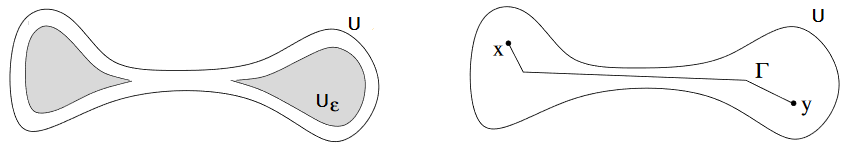
\includegraphics[scale=0.7]{Connected.png}
\caption{If $U$ is connected then its subdomain $U_{\varepsilon}$ may not be connected. However, any two points $x,y\in U$ can be connected by a polygonal path $\Gamma$ remaining inside $U$. So, if $\varepsilon >0$ is sufficiently small, then $x$ and $y$ belong to the same connected component of $U_{\varepsilon}$.}
\end{center}
\end{figure}

Let $\delta=\underset{z\in\Gamma}{\min} ~d(z,\partial U)$ be the minimum distance of points in $\Gamma$ to the boundary of $U$. Then for every $\varepsilon < \delta$ the whole polygonal  curve $\Gamma$  is  in  $U_{\varepsilon}$. So $x,y$ lie  in  the  same connected  component  of  $U_{\varepsilon}$. Hence $u_{\varepsilon}(x)=u_{\varepsilon}(y)\equiv \text{const}.$
\\
\bigskip
As $u\in W^{1,p}(U)$, Theorem 7 in Appendix C of Evans tells us that
$$u_{\varepsilon}\overset{\varepsilon \to0}{\longrightarrow } u ~\text{a.e. in $U$}.$$
Thus, $u$ is a constant a.e. in $U$.
\end{proof}
\phantomsection
\subsection{\textbf{5.10.13}} Give an example of an open set $U\subset \mathbb R^n$ and a function $u\in W^{1,\infty}(U)$, such that $u$ is \textit{not} Lipschitz continuous on $U$. (Hint: Take $U$ to be the open unit disk in $\mathbb R^2$, with a slit removed).

\begin{proof}
Consider the slit plane
$$A=\{(r,\theta):0< r < \infty,~ -\pi < \theta < \pi\}\subset\mathbb R^2,$$
in polar coordinates. The function 
$$u(r,\theta)=r\sin\left(\frac{\theta}{2}\right)$$
is continuous and locally Lipschitz. However, if we let $\varepsilon > 0$ and define a compact subset of $A$ as
$$K=\{(r,\theta): 1/2 \le r \le 3/2,~ -\pi + \varepsilon \le \theta \le \pi - \varepsilon \}\subset\mathbb R^2,$$
then we will see that the Lipschitz constant will be unbounded. Define $r=1$ and $\theta =\pm (\pi - \varepsilon)$ and consider two points in $K$ where $x_1(r,\theta)=(1,\pi-\varepsilon)$ and $x_2(r,\theta)= (1, \varepsilon - \pi).$ Then when $\varepsilon \to 0^+$
\begin{align*}
    \sup_{x_1 \ne x_2} \frac{|u(x_1)-u(x_2)|}{|x_1 - x_2|} &\ge
    \lim_{\varepsilon \to 0^+}\frac{\left|\sin\left(\frac{\pi - \varepsilon}{2}\right)- \sin\left(\frac{\varepsilon - \pi}{2}\right)\right|}{\left|\cos(\pi - \varepsilon)-\sin(\varepsilon-\pi)\right|}\\&=
    \lim_{\varepsilon \to 0^+}\frac{2\cos\left(\varepsilon /2\right)}{\sin(\pi-\varepsilon)} \\& \to \infty.
\end{align*}
Thus when $\varepsilon \to 0^+$ we see that the Lipschitz constant is unbounded. Therefore $u\in W^{1,\infty}(U)$ is not Lipschitz continuous.

\end{proof}


\phantomsection
\subsection{\textbf{5.10.15}} Fix $\alpha > 0$ and let $U=B^0(0,1)$. Show that there exists a constant $C$, depending only on $n$ and $\alpha$, such that
$$\int_U u^2\,dx \le C\int_U |Du|^2 \,dx,$$
provided
$$\left|\{x\in U~|~u(x)=0\}\right| \ge \alpha, \quad u\in H^1(U).$$

 My analysis closely follows the ideas presented by Giovanni Leoni in Chapter $12$ of \cite{article}. I will show that a variant of the Poincaré inequality is true in $W^{1,2}(U)$.

\begin{theorem}[Poincaré inequality in $W^{1,2}(U)$] Let $p=2$ and let $U\subset\mathbb R^2$ be a connected extension domain for $W^{1,2}(U)$ with finite measure. Let $E\subset U$ be a Lebesgue measurable set with positive measure. Then there exists a constant $C=C(2,U,E)>0$ such that for all $u\in W^{1,2}(U)$,   \begin{equation}\int_U|u(x)-u_E|^2\,dx\leq C\int_U|Du(x)|^2\,dx,\end{equation}
where  $$  u_E:=\frac{1}{|E|}\int_E u(x)\,dx=\frac{1}{\mathcal{L}^N(E)}\int_E u(x)\,dx.$$
\end{theorem}
\begin{proof}
 Let $E:=\{x\in U~|~u(x)=0\}$. Then $|E|>0$ and  $u_E=0$ by definition. Assume by contradiction that the result is false. Then, there exists a sequence $(u_n)\subset H^1(U)=W^{1,2}(U)$ such that
 $$\int_U \left|u_n(x)-(u_n)_E\right|^2 \,dx > n\int_U |Du_n(x)|^2\,dx>0.$$
 Define
 \begin{equation}v_n:=\frac{u_n-(u_n)_E}{\norm{u_n-(u_n)_E}_{L^2(U)}},\end{equation}
 then $v_n\in W^{1,2}(U)$ and 
 $$\norm{v_n}_{L^2(U)}=1,\quad (v_n)_E=0,\quad \int_U |Dv_n|^2\,dx < \frac{1}{n},$$
 where the last statement follows from
 $$\norm{Dv_n}_{L^2(U)}^2 < \frac{1}{n}\norm{v_n}_{L^2(U)}^2.$$
 By the Rellich–Kondrachov Compactness theorem, there exists a subsequence $(v_{n_k})$ such that $v_{n_k}\to v$ in $L^2(U)$ for some function $v\in L^2(U)$. So $(2)$ and the definition of $u_E$ imply
 $$\norm{v}_{L^2(U)}=1,\quad v_E=0.$$
 Therefore for every $\phi\in C_c^1(U)$ and $i=1,2,\ldots,N$ we find by Hölder's inequality
 \begin{align*}
     \left|\int_U v\frac{\partial \phi}{\partial x_i}\,dx\right|&=\lim_{k\to\infty}\left|\int_U v_{n_k}\frac{\partial \phi}{\partial x_i}\,dx\right|=\lim_{k\to\infty}\left|\int_U \frac{\partial v_{n_k}}{\partial x_i}\phi\,dx\right|\\&\le
     \lim_{k\to\infty}\left(\int_U \left|Dv_{n_k}\right|^2\,dx\right)^{1/2}\left(\int_U \left|\phi\right|^2\,dx\right)^{1/2}\\&
     \to 0,
 \end{align*}
Consequently $v\in W^{1,2}(U)$ where $Dv=0$ a.e. As $U$ is connected, $v$ must be a constant (see $5.10.11$). However, as $v_E=0$ and $v$ is a constant, we see that $v = 0$. This is a direct contradiction to the fact that $\norm{v}_{L^2(U)}=1$ and completes the proof. As $u_E=0$, $(1)$ implies that result is true for $5.10.15$.
\end{proof}
\phantomsection
\subsection{\textbf{5.10.17}} (Chain Rule) Assume $F:\mathbb R \to \mathbb R$ is $C^1$, with $F'$ bounded. Suppose $U$ is bounded and $u\in W^{1,p}(U)$ for some $1\le p \le \infty$. Show
$$v:=F(u)\in W^{1,p}(U)\quad\text{and}\quad v_{x_i}=F'(u)u_{x_i}\quad (i=1,\ldots,n).$$
(Hint: Use that any sequence that converges in $L^p$ has a subsequence that converges pointwise a.e.)

\begin{proof} \textbf{First Solution:} 
Let $u\in W^{1,p}(U)$. There exists $u_k\in C^{\infty}(U)\cap W^{1,p}(U)$ such that
$$\norm{u-u_k}_{W^{1,p}(U)}\to 0$$
as $k\to\infty$. Now
$$\left|F(u_k)(x) - F(u_\ell)(x)\right|\leq C|u_k(x)-u_\ell(x)|$$
since $F'$ is bounded. Moreover
$$DF(u_k)(x) =F'(u_k)(x)Du_k(x).$$
From this it follows that for any test function $\phi\in C_c^{\infty}(U)$
$$\int F(u)D\phi\,dx = \lim_{k\to\infty}\int F(u_k)D\phi\,dx = -\lim_{k\to\infty}\int F'(u_k)Du_k\phi\,dx.$$
We may choose a subsequence so that $u_k$ tends a.e. to $u$ and hence $F'(u_k)$ a.e. to $F'(u)$. Now
\begin{align*}
    &\left|\int \big(F'(u_k)Du_k - F'(u)Du\big)\phi\,dx \right|\\&=
    \left|\int \Big(\big(F'(u_k) - F'(u)\big)Du_k + F'(u)\big(Du_k - Du\big)\Big)\phi\,dx\right|\\&\leq
    C\int \Big(\norm{Du_k}_{\infty}\left|F'(u_k)-F(u)\right| + \norm{F'(u)}_{\infty}\norm{u_k - u}_{W^{1,p}(U)}\Big)|\phi|\,dx
\end{align*}
which tends to zero. Hence
$$\int F(u)D\phi\,dx = -\int F'(u)Du\phi\,dx.$$
Since $U$ is bounded $F(u)\in L^p(U)$ and since $F'(U)$ is bounded $F'(U)u_{x_i}\in L^p(U)$ and hence $F(u)\in W^{1,p}(U)$.

\textbf{Second Solution:} We assume $1\le p < \infty$. Let $\phi\in C_c^{\infty}(U)$. By the density theorem, there is a sequence $(u_n)\subset C^{\infty}(U)$ such that $u_n\to u$ in $W^{1,p}(U)$. Therefore, $u_n\to u$ and $Du_n \to Du$ a.e. in U. Defining $v_n=F(u_n)$, we see that both $F,u_n \in C^1$, so $v_n\in C^1$. This implies that we may use the chain rule for smooth functions to form
\begin{equation}-\int_U F(u_n)\frac{\partial \phi}{\partial x_i}\,dx = \int_U F'(u_n)\frac{\partial u_n}{\partial x_i}\phi\,dx.\end{equation}
As $F'$ is bounded, we let $M=\underset{t\in\mathbb R}\sup|F'(t)|$. Then
$$\left|\int_U \left(F(u_n)-F(u)\right)\frac{\partial \phi}{\partial x_i}\,dx\right|\le \norm{\frac{\partial \phi}{\partial x_i}}_{L^{\infty}} ~M \int_U |u_n - u|\,dx~ {\to}~ 0~~\text{as $n\to\infty$},$$
because $u_n \to u$ a.e. in $U$. Also
\begin{align*}
    \left|\int_U \left(F'(u_n)\frac{\partial u_n}{\partial x_i}-F'(u)\frac{\partial u}{\partial x_i}\right)\phi\,dx\right|&\le
    \norm{\phi}_{L^{\infty}}\int_U \Big|F'(u_n)\Big|\cdot\Big|\frac{\partial u_n}{\partial x_i} - \frac{\partial u}{\partial x_i}\Big|\,dx \\&+
    \norm{\phi}_{L^{\infty}}\int_U \Big|F'(u_n)-F'(u)\Big|\cdot\Big|\frac{\partial u}{\partial x_i}\Big|\,dx,
\end{align*}
where
$$\int_U \Big|F'(u_n)\Big|\cdot\Big|\frac{\partial u_n}{\partial x_i} - \frac{\partial u}{\partial x_i}\Big|\,dx  \le M \int_U \Big|\frac{\partial u_n}{\partial x_i} - \frac{\partial u}{\partial x_i}\Big|\,dx~ {\to}~ 0~~\text{as $n\to\infty$}.$$
Similarly, since $F'(u_n) \to F'(u)$ pointwise a.e. and 
$$\Big|F'(u_n)-F'(u)\Big|\cdot\Big|\frac{\partial u}{\partial x_i}\Big|\le 2M \Big|\frac{\partial u}{\partial x_i}\Big|,$$
we apply the dominated convergence theorem to conclude
$$\int_U \Big|F'(u_n)-F'(u)\Big|\cdot\Big|\frac{\partial u}{\partial x_i}\Big|\,dx ~ {\to}~ 0~~\text{as $n\to\infty$}.$$
Together, these imply
$$ \left|\int_U \left(F'(u_n)\frac{\partial u_n}{\partial x_i}-F'(u)\frac{\partial u}{\partial x_i}\right)\phi\,dx\right|~ {\to}~ 0~~\text{as $n\to\infty$}.$$
We now take $n\to\infty$ in $(3)$ to obtain
\begin{equation}-\int_U F(u)\frac{\partial \phi}{\partial x_i}\,dx = \int_U F'(u)\frac{\partial u}{\partial x_i}\phi\,dx,\end{equation}
which is the desired form of $v_{x_i}=F'(u)u_{x_i}$. As both $F$ and $u$ are sufficiently smooth, it follows that the right-hand side of $(4)$ is in $L^p(U)$, which implies that $v_{x_i}\in L^p(U)$. To see that $v\in W^{1,p}(U)$, we may observe
$$\int_U |v|^p\,dx = \int_U \left|F(u)-F(0)\right|^p\,dx \le M^p \int_U |u|^p < \infty.$$
For $p=\infty$, we review Chapter 5.8 of Evans. Let $U$ be open and bounded, with $\partial U$ of class $C^1$. Then $u: U\to \mathbb{R}$ is Lipschitz continuous $\iff$ $u\in W^{1,\infty}(U)$. Therefore, $W^{1,\infty}(U)$ is the space of Lipschitz continuous functions in $U$. So for every $x,y\in U$
$$ \left|F(u(x))-F(u(y))\right|= \left|\int_{u(y)}^{u(x)}F'(t)\,dt \right|\le M |u(x)-u(y)|.$$
Then, since $u$ is a Lipschitz function it must have Lipschitz constant, say $|u(x)-u(y)| \le L |x-y|$ for every $x,y\in U$. This implies
$$ \left|F(u(x))-F(u(y))\right| \le ML  |x-y|,$$
which shows that $v=F(u)\in W^{1,\infty}(U)$. Theorem 6 in Section 5.8 of Evans is known as Rademacher's Theorem. It states that if $u$ is locally Lipschitz continuous in $U$ then $u$ is differentiable almost everywhere in $U$. As we have shown that $v=F(u)$ is locally Lipschitz continuous, it follows that $v_{x_i}=F'(u)u_{x_i}$ as in the case when $1\le p < \infty$.

\end{proof}
\phantomsection
\subsection{\textbf{5.10.18}} Assume $1\le p\le \infty$ and $U$ is bounded.
\begin{enumerate}[label=(\alph*)]
    \item Prove that if $u\in W^{1,p}(U)$, then $|u|\in W^{1,p}(U)$.
    \item Prove $u\in W^{1,p}(U)$ implies $u^+,u^-\in W^{1,p}(U),$ and
    $$Du^+=\begin{cases} 
      Du & \text{a.e. on $\{u > 0\}$} \\
      0 & \text{a.e. on $\{u\le 0\}$},
   \end{cases}$$
   $$Du^-=\begin{cases} 
      0 & \text{a.e. on $\{u \ge 0\}$} \\
      -Du & \text{a.e. on $\{u < 0\}$}.
   \end{cases}$$
   (Hint: $u^+ = \lim_{\varepsilon\to 0}F_{\varepsilon}(u),$ for
   $$F_{\varepsilon}(z):=\begin{cases} 
      (z^2+\varepsilon^2)^{1/2}-\varepsilon& \text{if $z\ge 0$} \\
      0 & \text{if $z<0$}.)
   \end{cases}$$
   \item Prove that if $u\in W^{1,p}(U),$ then
   $$Du = 0 \text{ a.e.}\quad \text{on the set $\{u=0\}$}.$$
\end{enumerate}
\begin{proof}
We need to show that if $u\in W^{1,p}(U)$, then $u^+, u^-,|u|\in W^{1,p}(U)$. By Appendix A.3 of Evans,
$$u^+=\max(u,0),\quad u^-=-\min(u,0).$$
Following the hint for $(b)$, we let 
$$F_{\varepsilon}(z)=\begin{cases} 
      \sqrt{z^2+\varepsilon^2}-\varepsilon,& \text{if $z\ge 0$}, \\
      0, & \text{if $z<0$,}
   \end{cases}$$
therefore $F_{\varepsilon}(z)\in C^1(\mathbb R)$ and
$$(F_{\varepsilon})'(z)=\begin{cases} 
      \dfrac{z}{\sqrt{z^2+\varepsilon^2}},& \text{if $z > 0$}, \\
      0, & \text{if $z\le 0$},\end{cases}$$
 which implies that $\norm{(F_{\varepsilon})'}_{L^{\infty}(\mathbb R)}\le 1$ for every $\varepsilon > 0$. Also, $F(z)=$ $\lim_{\varepsilon\to 0}F_{\varepsilon}(z)$, where
 $$F(z)=\begin{cases} 
      z,& \text{if $z\ge 0$}, \\
      0, & \text{if $z<0$.}
   \end{cases}$$
The conditions of the chain rule for $W^{1,p}$ are satisfied and we have
$$\int_U F_{\varepsilon}(u)\frac{\partial \phi}{\partial x_j}\,dx = -\int_U (F_{\varepsilon})'(u)\frac{\partial u}{\partial x_j}\phi\,dx,$$
for every $\phi\in C_0^{\infty}(U)$. Observing that
$$\lim_{\varepsilon\to 0}(F_{\varepsilon})'(u)=\begin{cases} 
      1,& \text{on $\{u> 0\}$}, \\
      0, & \text{on $\{u\le0\}$},\end{cases}$$
and
$$u^+ = \lim_{\varepsilon\to 0}F_{\varepsilon}(u)\quad \text{in $U$},$$
we apply the dominated convergence theorem $\left(\norm{(F_{\varepsilon})'}_{L^{\infty}(\mathbb R)}< \infty\right)$ as in $5.10.17$ to find
\begin{align*}
    \int_U u^+ \frac{\partial \phi}{\partial x_j}\,dx&=
    \int_U \lim_{\varepsilon\to 0}F_{\varepsilon}(u) \frac{\partial \phi}{\partial x_j}\,dx\\&=
    \lim_{\varepsilon\to 0} \int_U F_{\varepsilon}(u) \frac{\partial \phi}{\partial x_j}\,dx\\&=
    - \lim_{\varepsilon\to 0} \int_U (F_{\varepsilon})'(u)\frac{\partial u}{\partial x_j}\phi\,dx \quad\text{(Chain Rule)}
    \\&=
    -\int_U \lim_{\varepsilon\to 0}(F_{\varepsilon})'(u)\frac{\partial u}{\partial x_j}\phi\,dx \quad\text{(DCT)}\\&=
    -\int_{u > 0}\frac{\partial u}{\partial x_j}\phi\,dx.
\end{align*}
This shows that $$Du^+=\begin{cases} 
      Du, & \text{a.e. on $\{u > 0\}$}, \\
      0, & \text{a.e. on $\{u\le 0\}$}.
   \end{cases}$$ 
As $u^- = (-u)^+$, an analogous argument will complete $(b).$ Then, $(a)$ follows from the fact that $|u|=u^+ + u^-$. 
\\
\bigskip
For $(c)$, we have 
$$u = u^{+} - u^{-} ~\implies~ \frac{\partial u}{\partial x_i}=\frac{\partial u^{+}}{\partial x_i}-\frac{\partial u^{-}}{\partial x_i} ,$$ 
therefore ${\partial u}/{\partial x_i}=0$ a.e. on $\{u=0\}$ and 

$$D|u|=\begin{cases} 
      Du, & \text{a.e. on $\{u > 0\}$}, \\
      0, & \text{a.e. on $\{u=0\}$},\\
      -Du, & \text{a.e. on  $\{u<0\}$}.
   \end{cases}$$ 
\end{proof}
\phantomsection
\subsection{\textbf{Exercise (Hardy's Inequality on $\mathbb R_+$)}} Let $p\in(1,\infty)$. Then there exists a constant $C=C(p) < \infty$ such that for $u\in W^{1,p}(U)$ with $Tu=0$,
$$\int_0^\infty \left| \frac1t \int_0^t f(s) \, ds\right|^p \, dt  \le \left(\frac p{p-1}\right)^p \int_0^\infty |f(s)|^p \, ds .$$

\begin{proof}
We will show 
\begin{equation}
\left(\int_0^\infty \left| \frac1t \int_0^t f(s) \, ds\right|^p \, dt \right)^{1/p} \le \frac p{p-1} \left(\int_0^\infty |f(s)|^p \, ds \right)^{1/p}.
\end{equation}
Observe that
$$ \frac1t \int_0^t f(s) \, ds = \int_0^1 f(t s) \, ds .$$
Therefore by applying Minkowski's integral inequality to the left hand side of $(5)$, we see
\begin{align*}
\left(\int_0^\infty \left| \int_0^1 f(t s) \, ds\right|^p \,dt\right)^{1/p} &
\le \int_0^1\left(\int_0^\infty \left|f(ts)\right|^p\,dt\right)^{1/p}\,ds \\&=
\int_0^1 s^{-1/p}\,ds\left(\int_0^\infty \left|f(t)\right|^p\,dt\right)^{1/p}
\\&=
\frac{p}{p-1}\left(\int_0^\infty \left|f(s)\right|^p\,ds\right)^{1/p},
\end{align*}
as required.

\end{proof}

\phantomsection
\section{Chapter 6 Solutions}

\phantomsection
\subsection{\textbf{6.6.3}} A function $u\in H_0^2(U)$ is a weak solution of this boundary-value problem for the \textit{biharmonic equation}
\[
  \begin{cases} 
      \Delta^2 u=f & \text{in $U$} \\
      u=\frac{\partial u}{\partial \nu}=0 & \text{on $\partial U$} 
   \end{cases}
   \tag{\ast} \label{eq:special}
\]
provided
$$\int_U\Delta u\Delta v \,dx = \int_U fv\,dx$$
for all $v\in H_0^2(U)$. Given $f\in L^2(U)$, prove that there exists a unique weak solution of $(\ast)$.

\begin{proof}
We first derive a variation of the Poincaré inequality. We have that $H_0^2(U):=\overline{C_c^{\infty}(U)}^{\norm{\cdot}_{2,2}}$. Therefore, if $u\in H_0^2(U)$ there exists a sequence $(u_n)\subseteq C_c^{\infty}(U)$ such that $u_n\to u \in W^{2,2}(U)$. Thus $H_0^2(U)$ consist of the functions $W^{2,2}(U)$ such that $u=0$ and $\nabla u =0$ on $\partial U$. As $u,\nabla u \in W_0^{1,2}(U)$ we see that both of the following Poincaré inequalities are true:
$$\norm{u}_{L^2(U)}\le C_1\norm{\nabla u}_{L^2(U)},$$
$$\norm{\nabla u}_{L^2(U)}\le C_2\norm{\nabla^2 u}_{L^2(U)},$$
where $C_1,C_2>0$. These two inequalities allow us to obtain a Poincaré inequality for the $H_0^2(U)$-norm
\begin{align*}
    \norm{u}_{H_0^2(U)} &= \norm{u}_{L^2(U)}^2 + \norm{\nabla u}_{L^2(U)}^2 + \norm{\nabla^2 u}_{L^2(U)}^2 \\&\le
    (1+C_1+C_2)\norm{\nabla^2 u}_{L^2(U)}^2 \\&=
    \tilde{C}\norm{\nabla^2 u}_{L^2(U)}^2.
\end{align*}
But we also have that
$$\norm{\nabla^2 u}_{L^2(U)}^2 \le \norm{u}_{H_0^2(U)}^2.$$
Therefore $\norm{\nabla^2 u}_{L^2(U)}^2$ is an equivalent norm in $H_0^2(U)$ and we think of 
\begin{equation} \norm{u}_{2,2}^2 =\norm{\nabla^2 u}_{L^2(U)}^2 \end{equation}
as our norm on $H_0^2(U)$. We now claim that
\begin{equation}
    \norm{\Delta u}_{L^2(U)}=\norm{\nabla^2 u}_{L^2(U)},
\end{equation}
for every $u\in H_0^2(U).$ To prove this, we consider $u\in C_c^{\infty}(U)$. Integrating by parts and commuting partial derivatives gives
$$\int_U u_{x_ix_i}u_{x_jx_j}\,dx = \int_U u_{x_ix_j}u_{x_ix_j}\,dx $$
for every $1\le i,j\le N$. We then sum over all $i$ and $j$ to arrive at
$$\norm{\Delta u}_{L^2(U)}= \norm{\nabla^2 u}_{L^2(U)}$$
for every $u\in C_c^{\infty}(U).$ As $C_c^{\infty}(U)$ is dense in $H_0^2(U)$, we pass to the limit to find
$$\norm{\Delta u}_{L^2(U)}=\norm{\nabla^2 u}_{L^2(U)},\quad \forall u\in H_0^2(U).$$
This proves $(7)$. Then $(6)$ implies that 
\begin{equation}\norm{u}_{H_0^2(U)}\le C\norm{\Delta u}_{L^2(U)}.\end{equation}
A similar analysis is shown in Stein: Singular integrals and Differentiability Properties of Functions \cite{10.2307/j.ctt1bpmb07}.
\\
\bigskip
For the biharmonic equation, we let $f\in L^2(U)$. We consider the bilinear form $B:H_0^2(U)\times H_0^2(U) \to \mathbb R$ defined by
$$B[u,v]:=\int_U \Delta u \Delta v \,dx \quad \forall u,v\in H_0^2(U),$$
and the linear functional $a:H_0^2(U)\to\mathbb R$ defined by
$$a(v):=\int_U fv\,dx \quad \forall v\in H_0^2(U).$$
We need to show that the hypotheses of the Lax-Milgram theorem are satisfied. First we observe that $B$ is continuous because
\begin{align*}
    |B[u,v]|&= \left|\int_U \Delta u \Delta v\,dx\right| \\&\le
    \left(\int_U |\Delta u|^2\,dx\right)^{1/2} \left(\int_U |\Delta v|^2\,dx\right)^{1/2}\\&\le
    C\norm{u}_{H_0^2(U)}\norm{v}_{H_0^2(U)},
\end{align*}
by the Cauchy-Schwarz inequality and the definition of the $H_0^2(U)$-norm. Moreover, $B$ is coercive as
$$B[u,u]=\int_U |\Delta u|^2\,dx = \norm{\Delta u}_{L^2(U)}^2\ge C\norm{u}_{H_0^2(U)}^2,$$
because of $(8)$. Also, the functional $a$ is continuous since
\begin{align*}
|a(v)| &\le \int_U |f||v|\,dx \\&\le 
\left(\int_U |f|^2\,dx\right)^{1/2}\left(\int_U |v|^2\,dx\right)^{1/2}\\&=
\norm{f}_{L^2(U)}\norm{v}_{L^2(U)} \\&\le
\gamma\norm{v}_{H_0^1(U)},
\end{align*}
where $\gamma := \norm{f}_{L^2(U)}$. Therefore, by the Lax-Milgram theorem we see that there exists a unique $u\in H_0^2(U)$ such that 
$$B[u,v]=a(v)\quad \forall v \in H_0^2(U).$$
Hence
$$\int_U \Delta u \Delta v \,dx = \int_U fv\,dx \quad \forall v\in H_0^2(U),$$
and the Lax-Milgram theorem provides a unique weak solution of $(\ast)$.

\end{proof}

\phantomsection
\subsection{\textbf{6.6.5}} Explain how to define $u\in H^1(U)$ to be a weak solution of Poisson's equation with $\textit{Robin boundary conditions}:$
\[
  \begin{cases} 
      -\Delta u=f & \text{in $U$} \\
      u+\frac{\partial u}{\partial \nu}=0 & \text{on $\partial U$}. 
   \end{cases}
\]
Discuss the existence and uniqueness of a weak solution for a given $f\in L^2(U)$.
\begin{proof}
To define a weak solution of Poisson's equation we multiply the equation by $v\in H^1(U)$ and integrate by parts to get
\begin{align*}
-\int_U \Delta u v \,dx &= \int_U D u \cdot D v \,dx - \int_{\partial U} v \frac{\partial u}{\partial \nu}\,dS \\&=
\int_U D u \cdot D v \,dx + \int_{\partial U} uv\,dS \\&=
\int_U fv\,dx.
\end{align*}
The boundary conditions imply that $u$ is a weak solution if
\begin{equation}
    \int_U D u \cdot D v \,dx + \int_{\partial U} (Tu)(Tv)\,dS = \int_U fv\,dx,
\end{equation}
where $u,v\in H^1(U)$ and $Tu=u|_{\partial U}$. We therefore define a weak solution to be a function $u\in H^1(U)$ which satisfies $(9)$ for all $v\in H^1(U)$. The Trace theorem tells us that the boundary conditions can be taken in the sense of traces.
\\
\bigskip
Let $f\in L^2(U)$. We will show that existence and uniqueness of a weak solution follow from the Lax-Milgram theorem. Analogously to $6.6.3$, the functional $a(v):=\int_U fv\,dv$ is continuous by the Cauchy-Schwarz inequality
\begin{align*}|a(v)| \le \int_U |f||v|\,dx &\le \norm{f}_{L^2(U)}\norm{v}_{L^2(U)} \\&\le \norm{f}_{L^2(U)}\norm{v}_{H^1(U)}\\&=\gamma \norm{v}_{H^1(U)}.
\end{align*}
We define the bilinear form $B:H^1(U)\times H^1(U)\to\mathbb R$ by
$$B[u,v]:=\int_U Du\cdot Dv\,dx +\int_{\partial U}(Tu)(Tv)\,dS\quad \forall u,v\in H^1(U).$$
We need to prove that the bilinear form is continuous and coercive. First, it is continuous by the  Cauchy-Schwarz inequality and the Trace inequality between $H^1(U)$ and $L^2(\partial U)$
\begin{align*}
    |B[u,v]| &\le \int_U |Du\cdot Dv| \, dx + \int_{\partial U}|(Tu)(Tv)|\,dS \\&\le
    \norm{Du}_{L^2(U)}\norm{Dv}_{L^2(U)} +  \norm{Tu}_{L^2(\partial U)} \norm{Tv}_{L^2(\partial U)} \\&\le
    (C+1)\norm{u}_{H^1(U)} \norm{v}_{H^1(U)}.
\end{align*}
To show that $B$ is coercive, assume by contradiction that it is not. Then there is a sequence $(u_n)\subset H^1(U)$ such that $\norm{u_n}_{H^1(U)}=1$ and $B[u_n,u_n]\to 0$. As $u_n$ is bounded in $H^1(U)$ and $H^1(U)$ is a Hilbert space, it contains a subsequence which converges weakly to $u\in H^1(U)$. Let's assume that $u_n \rightharpoonup u$. As $\partial U$ is Lipschitz, we have that $H^1(U) \subset L^2(U)$ and therefore $u_n\to u$ in $L^2(U)$ and $Du_n \rightharpoonup Du \in L^2(U)$.  
\\
\bigskip
As $B[u_n,u_n]\to 0$, we see that
\begin{equation}
 B[u_n,u_n] = \int_U |Du_n|^2\,dx +\int_{\partial U} Tu_n^2\,dS \to 0,   
\end{equation}
this implies that
$$\int_U |Du|^2\,dx \le \liminf_{n\to\infty} \int_U |Du_n|^2\, dx \to 0.$$
So by $5.10.11$ we know that $u$ is a constant. Now,
$$\lim_{n\to\infty}\int_U u_n^2 \,dx = \int_U u^2 \,dx=1.$$
However, since $Tu_n\to Tu$ in $L^2(\partial U)$, we see from $(10)$
$$\int_{\partial U} Tu^2 \,dS = \lim_{n\to\infty}\int_{\partial U} Tu_n^2\, dS \to 0 .$$
Therefore, as $u$ is a constant it cannot be both $0$ at the boundary and $1$ inside $U$. We have reached a contradiction and conclude that $B$ is coercive. The Lax-Milgram theorem then gives a unique weak solution to Poisson's equation.
\end{proof}
\phantomsection
\subsection{\textbf{6.6.7}} Let $u\in H^1(\mathbb R^n)$ have compact support and be a weak solution of the semilinear PDE
$$-\Delta u + c(u)=f\quad \text{in $\mathbb R^n$,}$$
where $f\in L^2(\mathbb R^n)$ and $c:\mathbb R \to \mathbb R$ is smooth, with $c(0)=0$ and $c'\ge 0$. Assume also $c(u)\in L^2(\mathbb R^n)$. Derive the estimate
$$\norm{D^2u}_{L^2} \le C\norm{f}_{L^2}.$$
(Hint: Mimic the proof of Theorem $1$ in §$6.3.1$, but without the cutoff function $\zeta$.)

\begin{proof}
Define $u\in H^1(\mathbb R^n)$ as a weak solution of the semilinear PDE 
\begin{equation}
\int_{\mathbb R^n} Du\cdot Dv \,dx = \int_{\mathbb R^n} fv\,dx - \int_{\mathbb R^n} c(u)v\,dx,
\end{equation}
provided that $v\in H^1(\mathbb R^n).$ As we have compact support, we are integrating over a large ball. Now let $h>0$ be small and choose $k\in\{1,\ldots,n\}$, and then substitute
$$v:=-D_k^{-h}(D_k^hu)$$
into $(11)$. This forms
\begin{equation*}
    -\underbrace{\int_{\mathbb R^n}Du\cdot D(D_k^{-h}(D_k^h u))\,dx}_{A} = -\underbrace{\int_{\mathbb R^n}fD_k^{-h}(D_k^hu)\,dx}_{B_1} + \underbrace{\int_{\mathbb R^n}c(u)D_k^{-h}(D_k^hu)\,dx}_{B_2}
\end{equation*}
The ``integration-by-parts'' formula for difference quotients is given in §$5.8.2$ in Evans by
$$\int_U u(D_k^h v)\,dx = -\int_U (D_k^{-h}u)v\,dx.$$
Applying this formula on $A$ gives
\begin{align*}
    A&=-\int_{\mathbb R^n} Du\cdot (D_k^{-h}(D_k^h(Du))\,dx \\&=
    \int_{\mathbb R^n} D_k^h(Du)\cdot D_k^h(Du)\,dx \\&=
    \int_{\mathbb R^n} |D_k^h(Du)|^2\,dx.
\end{align*}
Then by Cauchy's inequality with $\varepsilon$ and Theorem $3$ in §$5.8.2$ of Evans
\begin{align*}
|B_1| &\le \int_{\mathbb R^n} |f|\cdot|D_k^{-h}(D_k^hu)|\,dx \\&\le
\varepsilon\int_{\mathbb R^n} |D_k^{-h}(D_k^hu)|^2\,dx + \frac{C}{\varepsilon}\int_{\mathbb R^n} |f|^2\,dx \\&\le
C_1 \varepsilon \int_{\mathbb R^n} |D_k^h(Du)|^2\,dx+ \frac{C}{\varepsilon}\int_{\mathbb R^n} |f|^2\,dx.
\end{align*}
For $B_2$ we first observe
$$|c(u)(x)| = \left|\int_0^{u(x)} c'(t)\,dt \right|\le |u(x)|\cdot\norm{c'}_{L^{\infty}},$$
therefore
\begin{align*}
|B_2| &\le \int_{\mathbb R^n} |c(u)|\cdot|D_k^{-h}(D_k^hu)|\,dx \\&\le
C_2 \varepsilon \int_{\mathbb R^n} |D_k^h(Du)|^2\,dx+ \frac{C}{\varepsilon}\norm{c'}_{L^{\infty}}^2 \norm{u}_{L^2}^2.
\end{align*}
Combining the bounds for $A,B_1,B_2$ gives
\begin{align*}\int_{\mathbb R^n} |D_k^h(Du)|^2\,dx &\le (C_1+C_2)\varepsilon\int_{\mathbb R^n} |D_k^h(Du)|^2\,dx \\ &+\frac{C}{\varepsilon}\int_{\mathbb R^n} |f|^2\,dx + \frac{C}{\varepsilon}\norm{c'}_{L^{\infty}}^2 \norm{u}_{L^2}^2.
\end{align*}
Taking $\varepsilon$ small enough so that it satisfies $(C_1+C_2)\varepsilon=\frac{1}{2}$ yields
$$\frac{1}{2}\int_{\mathbb R^n} |D_k^h(Du)|^2\,dx \le \frac{C}{\varepsilon}\left(\norm{f}_{L^2}^2 + \norm{c'}_{L^{\infty}}^2 \norm{u}_{L^2}^2\right).$$
The above analysis holds for every $k\in\{1,\ldots,n\}$ and $h>0$ small. Therefore we apply Theorem $3$ in  §$5.8.2$ of Evans to conclude
$$\int_{\mathbb R^n} |D^2u|^2 \,dx\le \tilde{C}\left(\norm{f}_{L^2}^2 +  \norm{u}_{L^2}^2\right). $$
Hence $Du\in H^1(\mathbb R^n)$, so $u\in H^2(\mathbb R^n)$. 

\end{proof}
\phantomsection
\subsection{\textbf{6.6.8}} Let $u$ be a smooth solution of the uniformly elliptic equation $Lu=-\sum_{i,j=1}^n a^{ij}(x)u_{x_i}u_{x_j}=0$ in $U$. Assume that the coefficients have bounded derivatives. 
Set $v:=|Du|^2+\lambda u^2$ and show that
$$Lv\le 0 \quad \text{in U}$$
if $\lambda$ is large enough. Deduce
$$\norm{Du}_{L^{\infty}(U)}\le C\left(\norm{Du}_{L^{\infty}(\partial U)}+\norm{u}_{L^{\infty}(\partial U)}\right).$$
\begin{proof}
We first show the inequality $Lv\le 0$ in U. Observe that
$$Lu=-\sum_{i,j=1}^n a^{ij}u_{x_i}u_{x_j}=0$$
implies
$$D(Lu)=-\sum_{i,j=1}^n Da^{ij}u_{x_i}u_{x_j} - \sum_{i,j=1}^n a^{ij}Du_{x_i}u_{x_j}=0.$$
Therefore
$$-\sum_{i,j=1}^n Da^{ij}u_{x_i}u_{x_j} = \sum_{i,j=1}^n a^{ij}Du_{x_i}u_{x_j}.$$
We then compute
\begin{align*}
Lv &= -\sum_{i,j=1}^n a^{ij}\Big(Du\cdot Du + \lambda u^2\Big)_{x_ix_j}    \\&=
-2\sum_{i,j=1}^n a^{ij}\Big(Du_{x_ix_j}\cdot Du + Du_{x_i}\cdot Du_{x_j} + \lambda uu_{x_ix_j}+ \lambda u_{x_i}u_{x_j}\Big)\\&=
-2\left(\sum_{i,j=1}^n a^{ij}Du_{x_ix_j}\cdot Du + \sum_{i,j=1}^n a^{ij}Du_{x_i}\cdot Du_{x_j} + \lambda u \sum_{i,j=1}^n a^{ij}u_{x_ix_j} +\lambda \sum_{i,j=1}^n a^{ij}u_{x_i}u_{x_j}\right)\\&=
-2\sum_{i,j=1}^n a^{ij}Du_{x_ix_j}\cdot Du - 2\sum_{i,j=1}^n a^{ij}Du_{x_i}\cdot Du_{x_j}-0-2\lambda\sum_{i,j=1}^n a^{ij}u_{x_i}u_{x_j}\\&=
2\sum_{i,j=1}^n Da^{ij}u_{x_i}u_{x_j}\cdot Du - 2\sum_{i,j=1}^n a^{ij}Du_{x_i}\cdot Du_{x_j}-2\lambda\sum_{i,j=1}^n a^{ij}u_{x_i}u_{x_j}\\&\le
2\norm{Da^{ij}}_{L^{\infty}(U)}|D^2u||Du|-2\theta|D^2u|^2 - 2\lambda\theta|Du|^2\\&\le
\norm{Da^{ij}}_{L^{\infty}(U)}\left(|D^2u|^2 + |Du|^2)-2\theta|D^2u|^2 - 2\lambda\theta|Du|^2\quad\text{(Cauchy inequality)}\\&=
(C_1-2\theta)|D^2u|^2 + (C_2-2\lambda\theta)|Du|^2\\&\le
0.
\end{align*}
Where the last inequality true provided 
$$\lambda \ge \frac{(C_1-2\theta)|D^2u|^2}{2\theta|Du|^2}+\frac{C_2}{2\theta},$$ and is obtained for large $\lambda$. We now apply the weak maximum principle to deduce that for large $\lambda >0$
\begin{align*}
    \norm{|Du|^2}_{L^{\infty}(U)} &\le \norm{|Du|^2+\lambda u^2}_{L^{\infty}(U)}\\&\le
    \norm{|Du|^2+\lambda u^2}_{L^{\infty}(\partial U)} \\&\le
    \norm{|Du|^2}_{L^{\infty}(\partial U)} + \lambda\norm{ u^2}_{L^{\infty}(\partial U)}\\&\le
    C\left(\norm{|Du|}_{L^{\infty}(\partial U)}+\norm{ u}_{L^{\infty}(\partial U)}\right)^2,
\end{align*}
which implies the desired inequality.
\end{proof}

\phantomsection
\subsection{\textbf{6.6.10}} Assume $U$ is connected. Use $(a)$ energy methods and $(b)$ the maximum principle to show that the only smooth solutions of the Neumann boundary-value problem

\[
  \begin{cases} 
      -\Delta u=0 & \text{in $U$} \\
      ~~~\frac{\partial u}{\partial \nu}=0 & \text{on $\partial U$} 
   \end{cases}
\]

are $u\equiv C$, for some constant $C$.

\begin{proof}
For $(a)$, we multiply the Neumann problem by a test function $v$ in $U$ to form
\begin{align*}
    0 = -\int_U \Delta u v\,dx &=
    -\int_{\partial U}\frac{\partial u}{\partial \nu}v\,dS +\int_U Dv\cdot Du \,dx \quad\text{(Green's formula)} \\&=
    \int_U Dv\cdot Du \,dx.
\end{align*}
Letting $u=v$ yields
$$\int_U |Du|^2\,dx =0,$$
which implies that $Du=0$ a.e. in $U$. As $U$ is connected, we know from $5.10.11$ that $u\equiv C$ a.e. in $U$ for some constant $C$.
\\
\bigskip
For $(b),$ assume by contradiction that $u$ is not a constant. Then there must be some $x^0$ where $u$ attains its maximum in $\bar{U}$. If $x^0\in U$, then the strong maximum principle implies that $u$ is constant in contradiction to our assumption. Therefore, the maximum can only be obtained at the boundary of $U$ and we conclude that $u(x^0)>u(x)$ for all $x\in U$. However, Hopf's lemma then implies that
$$\frac{\partial u}{\partial \nu}(x^0)>0$$
in contradiction to $\frac{\partial u}{\partial \nu}=0$ on $\partial U$. So $u$ must obtain its maximum inside $U$ and the strong maximum principle implies that $u\equiv C$.
\end{proof}



\phantomsection
\subsection{\textbf{6.6.13}} (Courant minmax principle) Let $L=-\sum_{i,j=1}^n (a^{ij}u_{x_i})_x_j$, where $((a^{ij}))$ is symmetric. Assume the operator $L$, with zero boundary conditions, has eigenvalues $0 < \lambda_1 < \lambda_2 \le \cdots$. Show
$$\lambda_k = \underset{S\in \sum_{k-1}}{\max} \underset{\begin{subarray}{c}
  u\in S^{\perp} \\
  \norm{u}_{L^2}=1
  \end{subarray}}{\min}B[u,u]\quad \text{(k=1,2,\ldots).}$$
Here $\sum_{k-1}$ denotes the collection of $(k-1)$-dimensional subspaces of $H_0^1(U)$.

\begin{proof}
Let $\lambda_k$ denote an eigenvalue and $\phi_k$ an eigenfunction. We will apply the theorem of compact, self-adjoint operators as in Appendix $D$ of Evans to select an orthonormal basis. By defining
$$\nu_k= \underset{S\in \sum_{k-1}}{\max} \underset{\begin{subarray}{c}
  u\in S^{\perp} \\
  \norm{u}_{L^2}=1
  \end{subarray}}{\min}B[u,u]\quad \text{(k=1,2,\ldots),}$$
we need to show that $\nu_k = \lambda_k$.
\\
\bigskip
Choose any subspace $S$ where $\dim S=k-1$. Then select
$$u = \sum_{j=1}^k c_j\phi_j$$
where $\phi_1,\ldots,\phi_k$ are orthonormal and every $\phi_j$ is an eigenfunction of $\lambda_j$ for $j=1,\ldots,k$. We will choose the numbers $c_j$ such that $u\neq 0$ and $u\in S^{\perp}$. We then select the basis $\{e_1,\ldots,e_{k-1}\}$ in $S$ and consider the system of equations where $u$ is orthogonal to $e_1,\ldots,e_{k-1}$ in $L^2(U)$
$$\sum_{j=1}^k c_j\langle \phi_j,e_i\rangle=0,\quad i=1,\dots,k-1.$$
By construction, the $c_1,\ldots,c_k$ form $k$ unknowns and the coefficients $\langle \phi_j,e_i\rangle$ form $k-1$ equations. Therefore there exists a nontrivial solution $d_1,\ldots,d_k$. So
$$u=\sum_{j=1}^k d_j\phi_j$$
is in $S^{\perp}$ and is nonzero and hence we may assume that it is normalized. Then
$$B[u,u]=\sum_{j=1}^k \lambda_j |c_j|^2$$
because the eigenfunctions are orthonormal. As the $\lambda_j$ are ordered in an increasing order we see that
$$B[u,u]\le \lambda_k \sum_{j=1}^k |c_j|^2=\lambda_k \norm{u}_{L^2}^2=\lambda_k.$$
Therefore
$$\underset{\begin{subarray}{c}
  u\in S^{\perp} \\
  \norm{u}_{L^2}=1
  \end{subarray}}{\min}B[u,u]\le \lambda_k,$$
As this holds for any subspace $S$,
$$\underset{S\in \sum_{k-1}}{\max} \underset{\begin{subarray}{c}
  u\in S^{\perp} \\
  \norm{u}_{L^2}=1
  \end{subarray}}{\min}B[u,u]\le \lambda_k.$$
So $\nu_k\le \lambda_k$. The converse inequality follows from choosing $S=\text{span}(u_1,\ldots,u_{k-1}).$ Since the eigenfunctions are orthonormal and normalized, the eigenvalues may be written as 
$$\underset{\begin{subarray}{c}
  u\in S^{\perp} \\
  \norm{u}_{L^2}=1
  \end{subarray}}{\min}B[u,u]= \lambda_k,$$
 which implies that
 $$\nu_k=\underset{S\in \sum_{k-1}}{\max} \underset{\begin{subarray}{c}
  u\in S^{\perp} \\
  \norm{u}_{L^2}=1
  \end{subarray}}{\min}B[u,u]\ge \lambda_k,$$
hence $\nu_k \ge \lambda_k$.
\end{proof}
\phantomsection
\subsection{\textbf{6.6.15}} (Eigenvalues and domain variations)  Consider a family of smooth, bounded domains $U(\tau)\subset \mathbb R^n$ that depend smoothly upon the parameter $\tau\in\mathbb R$. As $\tau$ changes, each point on $\partial U(\tau)$ moves with velocity \textbf{v}.
For each $\tau$, we consider eigenvalues $\lambda = \lambda(\tau)$ and the corresponding eigenfunctions $w=w(x,\tau):$

\[
  \begin{cases} 
      -\Delta w=\lambda w & \text{in $U(\tau)$} \\
      ~~~~w=0 & \text{on $\partial U(\tau)$}, 
   \end{cases}
\]
normalized so that $\norm{w}_{L^2}(U(\tau))=1$. Suppose that $\lambda$ and $w$ are smooth functions of $\tau$ and $x$.
Prove \textit{Hadamard's variational formula}
$$\dot{\lambda}=-\int_{\partial U(\tau)}\left|\frac{\partial w}{\partial \nu}\right|^2 v\cdot \nu\,dS,$$
where $\cdot = \frac{d}{d\tau}$ and $v\cdot\nu$ is the normal velocity of $\partial U(\tau)$.
(Hint: Use the calculus formula from §$C.4.$)
\begin{proof}
Let $w=w(x,\tau)$ and $\norm{w}_{L^2}(U(\tau))=1$. Then
\begin{align*}\lambda(\tau)=\lambda(\tau)\cdot \norm{w}_{L^2}(U(\tau))&=\lambda(\tau)\int_{U(\tau)}|w|^2\,dx\\&=
\int_{U(\tau)}(-\Delta w)w\,dx\\&=
\int_{U(\tau)}|\nabla w|^2\,dx.
\end{align*}
By §$C.4$ in Evans,
\begin{align*}
\dot{\lambda}(\tau)&=\frac{d}{d\tau}\int_{U(\tau)}|\nabla w|^2\,dx \\&=
\int_{\partial U(\tau)} |\nabla w|^2 v\cdot \nu\,dS + \int_{U(\tau)} \left(|\nabla w|^2\right)_{\tau}\,dx \\&=
\int_{\partial U(\tau)} |\nabla w|^2 v\cdot \nu\,dS + \int_{U(\tau)} 2\nabla w \nabla w_{\tau} \,dx\\&=
\int_{\partial U(\tau)} |\nabla w|^2 v\cdot \nu\,dS + \int_{U(\tau)} 2w(-\Delta w_{\tau})\,dx \quad\text{(Integrate by parts)}.
\end{align*} 

To simplify the second integral, we see that
$$-\Delta w_{\tau}=(\lambda(\tau) w)_{\tau}=\lambda(\tau) w_{\tau}+\dot{\lambda}(\tau)w$$
and because $w=0$ on $\partial U(\tau)$
\begin{align*}0=\frac{d}{d\tau}\norm{w}_{L^2}(U(\tau))&=\frac{d}{d\tau}\int_{U(\tau)}|w|^2\,dx \\&= \int_{\partial U(\tau)}|w|^2 v\cdot \nu\,dS + \int_{U(\tau)}\left(|w|^2\right)_{\tau}\,dx\\&=\int_{U(\tau)}\left(|w|^2\right)_{\tau}\,dx\\&=
2\int_{U(\tau)}ww_{\tau}\,dx.
\end{align*}
Therefore
\begin{align*}
\dot{\lambda}(\tau)&=\int_{\partial U(\tau)} |\nabla w|^2 v\cdot \nu\,dS + \int_{U(\tau)} 2w\left(\lambda(\tau) w_{\tau}+\dot{\lambda}(\tau)w\right)\,dx \\&=
\int_{\partial U(\tau)} |\nabla w|^2 v\cdot \nu\,dS + 2\lambda(\tau)\int_{U(\tau)}ww_{\tau}\,dx + 2\dot{\lambda}(\tau)\int_{U(\tau)}w^2\,dx\\&=
\int_{\partial U(\tau)} |\nabla w|^2 v\cdot \nu\,dS +2\dot{\lambda}(\tau).
\end{align*}
The boundary condition $w=0$ on $\partial U(\tau)$ implies $|\nabla w|^2$ is equivalent to $\left|\frac{\partial w}{\partial \nu}\right|^2$ because the gradient is perpendicular to the boundary. This yields
$$-\dot{\lambda}(\tau)=\int_{\partial U(\tau)} \left|\frac{\partial w}{\partial \nu}\right|^2 v\cdot \nu\,dS,$$
as required.
\end{proof}
\phantomsection
\subsection{\textbf{Elasticity Exercise}} The homogeneous Dirichlet boundary conditions, reads
\[\begin{equation}
  \begin{cases} 
      -\text{div}Ae(u)=f & \text{in $U$} \\
      \qquad\qquad u=0 & \text{at $\partial U$} 
   \end{cases}.
   \end{equation}
\]
The unknown is a map $u:U\to\mathbb R^n$ which represents the displacement of an elastic body to which a force $f:U\to\mathbb R^n$ is applied. Here, as usual, $U\subset\mathbb R^n$ is an open and bounded domain. The notation $e(u) = \text{sym Du}$ stands for the symmetric part of the matrix of first partial derivatives of $u$. In components,
$$e_{ij}(u)=\frac{1}{2}(\partial_i u_j + \partial_j u_i),\quad i,j=1,\ldots,n.$$
The quantity $A= (a_{ijkl})$ encodes the elastic properties of the material and can depend on the spatial coordinate $x=(x_1,\ldots,x_n).$ It is a fourth order tensor defined using the indices $i,j,k,l\in\{1,\ldots,n\}$ so that, in the end, the PDE in $(7)$ denotes the system of equations
$$-\sum_{j,k,l=1}^n \partial_j(a_{ijkl}e_{kl}(u))=f_i,\quad i=1,\ldots,n.$$
Due to physical reasons, one typically has the symmetries
$$a_{ijkl}=a_{jikl},\quad a_{ijkl}=a_{ijlk},\quad a_{ijkl}=a_{klij}$$
for all choices of the indices, as well as the Legendre–Hadamard conditions
$$\sum_{i,j,k,l=1}^n a_{ijkl} \xi_i \xi_j p_k p_l \ge \lambda |\xi|^2 |p|^2 \quad \forall ~\xi,p\in\mathbb R^n$$
for some $\lambda \in(0,\infty).$ These ensure the system is uniformly elliptic. Assume throughout that $a_{ijkl}\in L^{\infty}(U)$.
\bigskip
\\
$(a)$ Let $f\in L^2(U;\mathbb R^n)$. Define an appropriate notion of weak solution for $(12)$, using the vectorial Sobolev space
$$H_0^1(U;\mathbb R^n)=\overline{C_c^{\infty}(U;\mathbb R^n)}$$
where the closure is taken with respect to the norm
$$\norm{u}_{H_0^1(U;\mathbb R^n)}=\sum_{i=1}^n \norm{u_i}_{H_0^1(U)}.$$

\begin{proof}
We first multiply $(12)$ by a test function $v$ and integrate over $U$
$$-\int_U\text{div}Ae(u)\cdot v\,dx=\int_U fv\,dx,\quad \text{for all $v\in H_0^1(U;\mathbb R^n)$.}$$
By the generalized form of Green's formula the LHS becomes
$$\int_U \text{div}Ae(u)\cdot v\,dx = \int_{\partial U} (Ae(u))\nu\cdot v\,dS - \int_U Ae(u):\nabla v\,dx,$$
where $\nu$ is the unit normal vector and
$$A:B = \sum_{i,j=1}^n A_{ij}B_{ij}.$$
Therefore
$$\int_U Ae(u):\nabla v\,dx - \int_{\partial U} (Ae(u))\nu\cdot v\,dS =\int_U fv\,dx.$$
The boundary condition of $u=0$ on $\partial U$ implies that the second integral on the LHS vanishes. Decomposing $A$ into its symmetric and anti-symmetric parts gives $A=(A+A^T)/2 + (A-A^T)/2$. This implies
\begin{align*}Ae(u):\nabla v &= Ae(u):\frac{1}{2}\left(\nabla v + \nabla v^T\right) + Ae(u):\frac{1}{2}\left(\nabla v - \nabla v^T\right)\\&=Ae(u):e(v).
\end{align*}
Therefore we have
$$\int_U Ae(u):e(v)\,dx=\int_U fv\,dx$$
as the weak form of $(12)$ where $v\in H_0^1(U;\mathbb R^n)$.
\end{proof}
$(b)$ Prove that weak solutions always exist for $f\in L^2(U;\mathbb R^n)$ and are unique. Hint: establish Korn’s inequality, which says that
$$C\int_U |e(u)|^2 \ge \int_U |Du|^2 \quad \forall~u\in H_0^1(U;\mathbb R^n)$$
for some constant $C\in(0,\infty).$
\begin{proof} Consider $B:H^1(U;\mathbb R^n)\times H^1(U;\mathbb R^n)\to \mathbb R$ where we define
$$B[u,v]=\int_U Ae(u):e(v)\,dx,$$
and $F:H^1(U;\mathbb R^n)\to\mathbb R$ where
$$\quad F(v)=\int_U fv\,dx.$$
Our problem is to find $u\in H^1(U;\mathbb R^n)$ such that
$$B[u,v]=F(v),\quad \text{for all $v\in H^1(U;\mathbb R^n)$.}$$
We will apply the Lax-Milgram theorem to show that weak solutions are unique and exist for $f\in L^2(U;\mathbb R^n)$. We first apply Hooke's law to write
$$Ae(u)=2\mu e(u)+\lambda(\nabla \cdot u)I,$$
where where $\mu > 0$ and $\lambda\ge$ 0 are called the Lamé constants. Then since $I:e(v)=\nabla \cdot v$ our bilinear form $B[u,v]$ becomes
$$B[u,v]=\int_U Ae(u):e(v)\,dx=2\mu(e(u):e(v))+\lambda(\nabla\cdot u, \nabla \cdot v).$$


We will show that $B$ is bounded. By the Cauchy-Schwarz inequality
\begin{align*}
    |B[u,v]| & = \left|2\mu(e(u):e(v))+\lambda(\nabla\cdot u, \nabla \cdot v)\right|  \\&\le
    2\mu\norm{e(u)}\norm{e(v)} + \lambda\norm{\nabla\cdot u}\norm{\nabla\cdot v} \\&\le
    C\norm{\nabla u}\norm{\nabla v}\\&\le
    \tilde{C}\norm{u}_{H_0^1(U;\mathbb R^n)}\norm{v}_{H_0^1(U;\mathbb R^n)}.
\end{align*}
Also, $F(v)$ is continuous through the Cauchy-Schwarz inequality
\begin{align*}
    |F(v)|&\le \norm{f}_{L^2}\norm{v}_{L^2} \\&\le
    \norm{f}_{L^2}\norm{v}_{H_0^1(U;\mathbb R^n)} \\&\le
    C\norm{v}_{H_0^1(U;\mathbb R^n)}.
\end{align*}
To show the coercivity for $B[u,v]$, we rely on the following
\begin{lemma}
(Korn's Inequality) There is a constant $C$ such that
$$C\norm{\nabla v}^2 \le \norm{e(v)}^2=\int_U \sum_{i,j=1}^n e_{ij}(v)e_{ij}(v)\,dx.$$
\end{lemma}
\textbf{Proof of Lemma:} As $u=0$ on $\partial U$, we calculate
\begin{align*}
\int_U \sum_{i,j=1}^n e_{ij}(v)e_{ij}(v)\,dx &=
\int_U \sum_{i,j=1}^n \frac{1}{2}\left(\frac{\partial v_i}{\partial x_j} + \frac{\partial v_j}{\partial x_i}\right)\frac{1}{2}\left(\frac{\partial v_i}{\partial x_j} + \frac{\partial v_j}{\partial x_i}\right)\,dx\\&=
\frac{1}{4}\int_U \sum_{i,j=1}^n \left(\frac{\partial v_i}{\partial x_j}\right)^2+2\frac{\partial v_i}{\partial x_j}\frac{\partial v_j}{\partial x_i}+ \left(\frac{\partial v_j}{\partial x_i}\right)^2\,dx\\&=
\frac{1}{2}\norm{\nabla v}^2 +\frac{1}{2}\sum_{i,j=1}^n\int_U \frac{\partial v_i}{\partial x_j}\frac{\partial v_j}{\partial x_i}\,dx.
\end{align*}
We then need to show that the last term on the RHS is positive. Integrating by parts and recognizing that $v=0$ on $\partial U$ gives
\begin{align*}
 \sum_{i,j=1}^n\int_U \frac{\partial v_i}{\partial x_j}\frac{\partial v_j}{\partial x_i}\,dx &=
 -\sum_{i,j=1}^n\int_U v_i\frac{\partial^2 v_j}{\partial x_i \partial x_j}\,dx + \int_{\partial U} \nu_j v_i \frac{\partial v_j}{\partial x_i}\,dS\\&=
 \sum_{i,j=1}^n\int_U \frac{\partial v_i}{\partial x_i}\frac{\partial v_j}{\partial x_j}\,dx - \int_{\partial U} \nu_i v_i \frac{\partial v_j}{\partial x_j}\,dS \\&=
 \left(\sum_{i=1}^n \frac{\partial v_i}{\partial x_i}\right)\left(\sum_{j=1}^n \frac{\partial v_j}{\partial x_j}\right)\,dx
 \\&= \int_U (\nabla \cdot v)^2\,dx \ge 0,
\end{align*}
as desired. Hence $\norm{e(v)}^2 \ge C \norm{\nabla v}^2$.
\bigskip
\\
Coercivity of $B[u,v]$ now follows from
\begin{align*}
    B[u,u] &= 2\mu \norm{e(u)}^2+\lambda \norm{\nabla\cdot u}^2 \\&\ge
    2\mu \norm{e(u)}^2 \\&\ge
    C \norm{\nabla u}^2 \\& \ge
    \tilde{C}\norm{u}_{H_0^1(U;\mathbb R^n)}^2.
\end{align*}
Therefore weak solutions for $f\in L^2(U;\mathbb R^n)$ exist and are unique by the Lax-Milgram theorem.

$(c)$ Prove the regularity theorem that if $A$ and $f$ are infinitely differentiable throughout $U$, then so must be the unique weak solution $u$.

\begin{proof}
By Hooke's law, we follow Ciarlet $\cite{ciarlet1994three}$ and rewrite the elasticity tensor as
\begin{equation}Ae(u)=\lambda(\text{tr}~e(u))I+2\mu e(u)\end{equation}
where once again $\mu > 0$ and $\lambda\ge$ 0 are called the Lamé constants. We then sketch a proof of the following
\begin{theorem}{(Regularity of weak solutions to the linear elasticity problem)}
Let $U$ be a domain in $\mathbb R^n$ with a boundary $\partial U$ of class $C^2$. Let $f\in L^p(U)$ and $p\ge 6/5$. Then the weak solution $u\in H_0^1(U)$ of the linear elasticity problem is in the space $W^{2,p}(U)$ and satisfies
$$-\text{div}\left(\lambda(\text{tr}~e(u))I+2\mu e(u)\right)=f \text{ in $L^p(U).$}$$
Furthermore, let $m\ge 1$ be an integer. If the boundary $\partial U$ is of class $C^{m+2}$ and if $f\in W^{m,p}$, then the weak solution $u\in H_0^1(U)$ is in the space $W^{m+2,p}(U)$.
\end{theorem}

\textbf{Sketch of proof:}
$(1)$ We will proceed similar to Theorem $2$ in §$6.3$ of Evans. The operator of linear elasticity is strongly elliptic because of the Legendre–Hadamard conditions. Therefore 
$$f\in L^2(U) \Longrightarrow u\in H^2(U)\cap H_0^1(U)$$
holds when the boundary $\partial U$ is of class $C^2$. This handles the regularity where $m=0$ and $p=2$. 
\bigskip
\\
$(2)$ Following the results of Agmon, Douglis, Nirenberg, and Geymonat, the uniform ellipticity condition gives the regularity result for $m=0$ and $p\ge 6/5$. I refer to Ciarlet $\cite{ciarlet1994three}$ as the details of this analysis are technical.
\bigskip
\\
$(3)$ By $(13)$, the weak solution $u\in W^{2,p}(U)\cap H_0^1(U)$ satisfies
\begin{equation}\int_U \left\{\lambda(\text{tr}~e(u))I+2\mu e(u)\right\}:e(v)\,dx=\int_U fv\,dx, \quad v\in H_0^1(U;\mathbb R^n).\end{equation}
We will apply Green's formula for Sobolev Spaces. Let $\nu=(\nu_i)$ be the outward unit normal vector for $\partial U$. Then for $i=1,2,\ldots,n$ Green's formula gives
$$\int_U (\partial_i u)v\,dx =-\int_U u \partial_i v\,dx +\int_{\partial U} uv \nu_i\,dS.$$
Applying the formula to the LHS of $(14)$ with Dirichlet boundary conditions yields
$$\int_U \left\{\lambda(\text{tr}~e(u))I+2\mu e(u)\right\}:e(v)\,dx=-\int_U\text{div}\left\{\lambda(\text{tr}~e(u))I+2\mu e(u)\right\}\cdot v\,dx,$$
by which we then conclude that $f\in W^{m,p}(U)$.
\bigskip
\\
$(4)$ After establishing the regularity result
$$f\in W^{m,p}(U) \Longrightarrow u\in W^{m+2,p}(U)$$
for $m=0$, we then apply the bootstrap argument to obtain higher regularity provided that the boundary $\partial U$ is of class $C^{m+2}$. Analagously to Theorem $6.3.2$ in Evans, we repeatedly apply Theorem $4$ for $m=0,1,2,\ldots$ to deduce infinite differentiability of $u$.


\end{proof}

\phantomsection
\section{Chapter 7 Solutions}
\phantomsection
\subsection{\textbf{7.5.1}} Prove that there is at most one smooth solution of this initial/boundary-value problem for the heat equation with Neumann boundary conditions
\[
  \begin{cases} 
      u_t-\Delta u=f & \text{in $U_T$} \\
      ~\qquad\frac{\partial u}{\partial \nu}=0 & \text{on $\partial U\times[0,T]$} \\
      ~~\qquad u = g & \text{on $U\times \{t=0\}$.}
   \end{cases}
\]

\begin{proof}
Let $u_1,u_2$ be solutions and define $w:=u_1-u_2$. Then the initial/boundary-value problem becomes
\[
  \begin{cases} 
      w_t-\Delta w=0 & \text{in $U_T$} \\
      ~\qquad\frac{\partial w}{\partial \nu}=0 & \text{on $\partial U\times[0,T]$} \\
      ~~\qquad w = 0 & \text{on $U\times \{t=0\}$.}
   \end{cases}
\]
We need to show that $w=0$. Define the energy to be
$$E(t):= \int_U \left(w(x,t)\right)^2 \,dx.$$
Differentiating under the integral sign yields
$$\frac{d}{dt}E(t)=2\int_U w(x,t)\cdot w_t(x,t)\,dx.$$
By the equation this expression equals
$$\frac{d}{dt}E(t)=2\int_U w(x,t)\cdot \Delta w(x,t)\,dx.$$
Through integration by parts in the $x$ variable, we deduce
\begin{align*}\frac{d}{dt}E(t)&=-2\int_U \left(Dw(x,t)\right)^2\,dx + 2\int_{\partial U} \frac{\partial w}{\partial \nu} w\,dS\\&=
-2\int_U \left(Dw(x,t)\right)^2\,dx \\& \le 0.
\end{align*}
Hence, $E(t)$ is decreasing in $t$.  In particular,  since $E(0) = 0$ and since $E(t)\ge 0$,  it follows that $E(t) = 0$ for all $t\ge 0$.  Hence, $w= 0$, as was claimed.
\end{proof}
\phantomsection
\subsection{\textbf{7.5.2}} Assume $u$ is a smooth solution of 
\[
  \begin{cases} 
      u_t-\Delta u=0 & \text{in $U_T \times (0,\infty)$} \\
      ~~\qquad u=0 & \text{on $\partial U\times[0,T]$} \\
      ~~\qquad u = g & \text{on $U\times \{t=0\}$.}
   \end{cases}
\]
Prove the exponential decay estimate
$$\norm{u(\cdot,t)}_{L_2(U)} \le e^{-\lambda_1 t}\norm{g}_{L^2(U)}\quad (t\ge 0),$$
where $\lambda_1$ is the principal eigenvalue of $-\Delta$ (with zero boundary conditions) on $U$.
\begin{proof}
As $u$ is a smooth solution of the initial/boundary-value problem we integrate by parts in the $x$ variable to obtain
\begin{align*}
\frac{d}{dt}\frac{1}{2}\norm{u(\cdot,t)}_{L_2(U)}^2 &=
\int_U u u_t\,dx\\&=
\int_U u \Delta u \,dx \\&=
-\int_U |Du|^2\,dx + \int_{\partial U}\frac{\partial u}{\partial \nu} u \,dS\\&=
-\int_U |Du|^2\,dx.
\end{align*}
From Theorem $2$ in $\S{6.5}$, we know that Rayleigh's formula is expressed as
$$\lambda_1 = \underset{\substack {u \in H_0^1 (U)\\ u\neq 0}}\min \frac{B[u,u]}{\norm{u}_{L^2(U)}^2} = 
\underset{\substack {u \in H_0^1 (U)\\ u\neq 0}}\min \frac{\int_U |Du|^2\,dx}{\norm{u}_{L^2(U)}^2},$$
where we may observe that $\frac{d}{dt}\frac{1}{2}\norm{u(\cdot,t)}_{L_2(U)}^2=-B[u,u]$ by the weak formation. This implies
$$\frac{d}{dt}\norm{u(\cdot,t)}_{L_2(U)}^2 \le -2\lambda_1\norm{u}_{L^2(U)}^2.$$
We now apply Gronwall's inequality to obtain the exponential decay estimate. Letting $\eta(t) = \norm{u(\cdot,t)}_{L_2(U)}^2$ we see that
$$\eta'(t)\le \phi(t)\eta(t)+\psi(t)$$
where $\phi(t)$ is a constant and $\psi(t)$ is zero. This gives
$$\eta(t)\le e^{\int_0^t \phi(s)\,ds}\eta(0)=e^{-2\lambda_1 t}\eta(0).$$
By the initial condition $u=g$ at $t=0$, we see that
$$\eta(0)=\norm{u(\cdot,0)}_{L_2(U)}^2=\norm{g}_{L_2(U)}^2.$$
This forms
$$\norm{u(\cdot,t)}_{L_2(U)}^2 \le e^{-2\lambda_1 t}\norm{g}_{L_2(U)}^2,$$
as desired.
\end{proof}
\phantomsection
\subsection{\textbf{7.5.5}} Assume
\[
  \begin{cases} 
      u_k \rightharpoonup u & \text{in $L^2(0,T;H_0^1(U))$}\\
      u'_k \rightharpoonup v & \text{in $L^2(0,T;H^{-1}(U))$}.
   \end{cases}
\]
Prove that $v=u'$. (Hint: Let $\phi\in C_c^1(0,T), w\in H_0^1(U).$ Then
$$\int_0^T \langle u'_k,\phi w\rangle \,dt = - \int_0^T \langle u_k,\phi' w\rangle \,dt.)$$

\begin{proof} As in $\S D.4$, $u_k \rightharpoonup u$ in $L^2(0,T;H_0^1(U))$ and $u'_k \rightharpoonup v$ in $L^2(0,T;H^{-1}(U))$ means
$$\int_0^T \langle u_k,h\rangle\,dt \to \int_0^T \langle u,h\rangle\,dt\quad \text{for all $h\in L^2(0,T;H^{-1}(U)),$}$$
$$\int_0^T \langle u_k',g\rangle\,dt \to \int_0^T \langle v,g\rangle\,dt\quad \text{for all $g\in L^2(0,T;H_0^1(U)),$}$$
 where $\langle~,~\rangle$ denotes the pairing between $H^{-1}(U)$ and $H_0^1(U)$. Following the hint, we let $\phi\in C_c^1(0,T), w\in H_0^1(U)$, and $g=\phi(t) w$. This implies that $g\in L^2(0,T,H_0^1(U))$. We then rewrite the above expressions as
\begin{equation}\int_0^T \langle u_k,\phi' w\rangle\,dt \to \int_0^T \langle u,\phi' w\rangle\,dt,\end{equation}
\begin{equation}\int_0^T \langle u_k',\phi w\rangle\,dt \to \int_0^T \langle v,\phi w\rangle\,dt.\end{equation}
Theorem $8$ (Bochner) in $\S E.5$ states that if $f:[0,T]\to X$ is strongly measurable then
$$\left\langle u^{\ast},\int_0^T f(t)\,dt\right\rangle = \int_0^T \left\langle u^{\ast},f(t)\right\rangle dt,$$
for every $u^{\ast}\in X^{\ast}$. We first deduce 
\begin{equation}\int_0^T \langle u, \phi' w\rangle \, dt = \int_0^T \langle u\phi' , w\rangle \, dt = \left\langle \int_0^T u(t)\phi'(t) \, dt , w\right \rangle,\end{equation}
and then observe
\begin{equation}\int_0^T \langle v, \phi w\rangle \, dt = \int_0^T \langle v\phi , w\rangle \, dt = \left\langle \int_0^T v(t)\phi(t) \, dt , w\right \rangle.\end{equation}
Combining $(17)$ and $(18)$ with the hint
$$\int_0^T \langle u'_k,\phi w\rangle \,dt = - \int_0^T \langle u_k,\phi' w\rangle \,dt$$
and taking the limit gives 
$$\left\langle \int_0^T u(t)\phi'(t) \, dt , w\right \rangle = \left\langle -\int_0^T v(t)\phi(t) \, dt , w\right \rangle$$
for every $w\in H^1_0(U)$. If we didn't want to use the hint, then we could observe by $(15)$ and $(16)$ that

\begin{align*}
\left\langle \int_0^T u(t)\phi'(t)\,dt,w \right\rangle &= 
\int_0^T \langle u\phi',w\rangle \,dt \\&=
\int_0^T \langle u,\phi' w\rangle \,dt \\&=
\lim_{k\to\infty} \int_0^T \langle u_k,\phi'w\rangle \,dt \\&=
\lim_{k\to\infty} \int_0^T \langle u_k\phi',w\rangle \,dt \\&=
\lim_{k\to\infty} \left\langle \int_0^T u_k(t)\phi'(t)\,dt,w\right\rangle \\&=
\lim_{k\to\infty} \left\langle -\int_0^T u'_k(t)\phi(t)\,dt,w\right\rangle\\&=
\lim_{k\to\infty} \int_0^T - \langle u'_k \phi,w\rangle \,dt\\&=
\lim_{k\to\infty} \int_0^T -\langle u'_k,\phi w\rangle \,dt\\&=
\int_0^T -\langle v,\phi w\rangle \,dt \\&=
\left\langle \int_0^T - v(t)\phi(t)\,dt, w\right\rangle.
\end{align*}
Both methods imply that
$$\int_0^T u(t)\phi'(t) \, dt = -\int_0^T v(t)\phi(t) \, dt$$ 
for every $\phi \in C_c^1(0,T)$. Hence, $v=u'$.
\end{proof}
\phantomsection
\subsection{\textbf{7.5.6}} Suppose $H$ is a Hilbert space and $u_k \rightharpoonup u$ in $L^2(0,T;H)$. Assume further we have the uniform bounds
$$\operatorname*{ess~sup}_{0\leq t\leq T}~\norm{u_k(t)}\le C \quad (k=1\ldots)$$
for some constant $C$. Prove 
$$\operatorname*{ess~sup}_{0\leq t\leq T}~\norm{u(t)}\le C.$$
(Hint: We have $\int_a^b(v,u_k(t))\,dt\le C\norm{v}|b-a|$ for $0\le a\le b \le T$ and $v\in H.$)
\begin{proof} Since $u_k \rightharpoonup u$ in $L^2(0,T;H)$ we know from $\S D.4$ that
$$\int_a^b(v,u_k(t))\,dt \to \int_a^b(v,u(t))\,dt, \quad \text{for all $v\in L^2(0,T;H).$}$$
Following the hint
$$\int_a^b(v,u_k(t))\,dt\le C\norm{v}|b-a|,\quad 0\le a\le b \le T,~ v\in H,$$
we let $k\to \infty$ to deduce
$$\int_a^b(v,u(t))\,dt\le C\norm{v}|b-a|.$$
Then since $|(v,u(t))|\le \norm{v}\norm{u(t)}$ by Cauchy–Schwarz we observe that taking the supremum where $\norm{v}\le 1$ gives
$$ \int_a^b\sup_{||v||\leq 1}|(v,u(t))|\,dt=\int_a^b \norm{u(t)}\,dt \le C|b-a|.$$
Hence $\norm{u(t)}\le C$ for all $0\le a\le b \le T$. This implies
$$\operatorname*{ess~sup}_{0\leq t\leq T}~\norm{u(t)}\le C.$$
\end{proof}
\phantomsection
\subsection{\textbf{7.5.12}} Prove the resolvent identities $(12)$ and $(13)$ in $\S7.4.1$.
\begin{proof}The requirement for $\lambda$ to be in the resolvent set is that the operator $\lambda I-A$ maps $D(A)$ bijectively onto $X$. As $\lambda,\mu \in p(A)$ we see that
$$\lambda I - A:D(A) \to X,\quad \mu I - A:D(A) \to X$$
are both bijective operators onto $X$ and are invertible. This implies that the operator times its inverse is the identity. By spectral theory,
$$R_{\lambda}(\lambda I - A)=(\lambda I - A)R_{\lambda} =I,$$
$$R_{\mu}(\mu I - A)= (\mu I - A)R_{\mu}= I.$$
Hence
\begin{align*}
    R_{\lambda}-R_{\mu} &= R_{\lambda} (\mu I-A) R_{\mu} - R_{\lambda}(\lambda I-A) R_{\mu} \\ &= 
    R_{\lambda} ((\mu I-A)-(\lambda I-A)) R_{\mu} \\&=
    R_{\lambda}(\mu - \lambda)R_{\mu} \\&=
    (\mu - \lambda)R_{\lambda}R_{\mu},
\end{align*}
which proves the first resolvent identity. The second identity follows from repeating the analysis and switching $\mu$ and $\lambda$. Then
\begin{align*}
    R_{\mu}-R_{\lambda} &= R_{\mu} (\lambda I-A) R_{\lambda} - R_{\mu}(\mu I-A) R_{\lambda} \\ &= 
    R_{\mu} ((\lambda I-A)-(\mu I-A)) R_{\lambda} \\&=
    R_{\mu}(\lambda - \mu)R_{\lambda} \\&=
    (\lambda- \mu)R_{\mu}R_{\lambda}.
\end{align*}
Therefore
$$R_{\lambda}R_{\mu}=\frac{R_{\lambda}-R_{\mu}}{\mu - \lambda}$$
and we have that
$$R_{\mu}R_{\lambda}=\frac{R_{\mu}-R_{\lambda}}{\lambda- \mu}=\frac{R_{\lambda}-R_{\mu}}{\mu - \lambda}=R_{\lambda}R_{\mu}.$$
\end{proof}
\phantomsection
\subsection{\textbf{7.5.13}} Justify the equality
$$A\int_0^{\infty}e^{-\lambda t}S(t)u\,dt = \int_0^{\infty} e^{-\lambda t}AS(t)u\,dt$$
used in $(16)$ of $\S7.4.1$. (Hint: Approximate the integral by a Riemann sum and recall that $A$ is a closed operator.)
\begin{proof}
$A$ is a closed means that whenever $u_k\in D(A)$ $(k=1,\ldots)$ and $u_k\to u, Au_k \to v$ as $k\to\infty$, then 
$$u\in D(A),\quad v=Au.$$
So we need to make a suitable choice for $u_k$. Following the hint in Evans, we look at the Laplace transform of the semigroup
$$\int_0^{\infty}e^{\lambda t}S(t)u\,dt$$
and approximate it by Riemann sums by letting
$$u_k = \sum_{i=1}^k e^{-\lambda t_i^*} S(t_i^*) u \Delta t,$$
where $t_{i-1}<t_i^* < t_i$ represent subintervals. By Theorem $1$ in $\S 7.4$ of Evans, $u\in D(A)$ implies that $S(t)u\in D(A)$ for every $t\ge 0$. As $\{S(t)\}_{t\ge 0}$ is a one-parameter family of linear operators, we see that $u_k \in D(A)$ because of the linearity of the operator $S(t)$. Furthermore, $A:D(A)\subset X \to X$ is also a linear operator. This implies that we can approximate the RHS of the equality
$$\int_0^{\infty} e^{-\lambda t}AS(t)u\,dt$$
by Riemann sums where
$$Au_k=\sum_{i=1}^k e^{-\lambda t_i^*} AS(t_i^*) u \Delta t.$$
Taking the limit as $k\to\infty$ yields
$$\lim_{k\to\infty}\sum_{i=1}^k e^{-\lambda t_i^*} S(t_i^*) u \Delta t = \int_0^{\infty}e^{\lambda t}S(t)u\,dt,$$
$$\lim_{k\to\infty}\sum_{i=1}^k e^{-\lambda t_i^*} AS(t_i^*) u \Delta t = \int_0^{\infty}e^{\lambda t}AS(t)u\,dt.$$
Therefore we see that as $k\to\infty$,
$$u_k \to \underbrace{\int_0^{\infty}e^{\lambda t}S(t)u\,dt}_{u}, \quad Au_k \to \underbrace{\int_0^{\infty}e^{\lambda t}AS(t)u\,dt}_{v}.$$
Since $A$ is closed, we know that $u\in D(A)$ and $v=Au$. Furthermore, since $A$ is linear we may conclude
$$\int_0^{\infty}e^{\lambda t}AS(t)u\,dt = A\int_0^{\infty}e^{\lambda t}S(t)u\,dt,$$
as required.
\end{proof}
\phantomsection
\subsection{\textbf{7.5.14}} Define for $t>0$
$$[S(t)g](x) = \int_{\mathbb R^n} \Phi(x-y,t)g(y)\,dy\quad (x\in\mathbb R^n),$$
where $g:\mathbb R^n \to \mathbb R$ and $\Phi$ is the fundamental solution of the heat equation. Also set $S(0)g=g$.
\\
\vspace{2px}
(a) Prove $\{S(t)\}_{t\ge 0}$ is a contraction semigroup on $L^2(\mathbb R^n).$
\\
\vspace{2px}
(b) Show $\{S(t)\}_{t\ge 0}$ is \textit{not} a contraction semigroup on $L^{\infty}(\mathbb R^n).$

\begin{proof}
For $(a)$ we know from $(9)$ in $\S 2.3$ of Evans that the fundamental solution of the heat equation in $\mathbb R^n$ may be written as the convolution
$$[S(t)g](x) = \frac{1}{(4\pi t)^{n/2}}\int_{\mathbb R^n} e^{-\frac{|x-y|^2}{4t}}g(y)\,dy$$
where $x\in\mathbb R^n,~t>0,~ g\in X$ for $X:=L^p(\mathbb R^n),~1\le p < \infty$. By defining
$$J_t(x):=(4\pi t)^{-n/2} e^{-|x|^2/{4t}},$$
we see that we can write
$$[S(t)g](x)=J_t * g(x).$$
A function $g:\mathbb R^n \to \mathbb R$ is said to be rapidly decreasing if it is infinitely many times differentiable $\left(g\in C^{\infty}(\mathbb R^n)\right)$ and
$$\lim_{|x|\to\infty} |x|^k D^{\alpha}g(x)=0\quad \text{for all $k\in\mathbb N$ and $\alpha\in\mathbb N^n.$}$$
The space
$$\mathscr{S}(\mathbb R^n):=\{g\in C^{\infty}(\mathbb R^n)~:~\text{$f$ is rapidly decreasing}\}$$
is called the Schwartz space. The function $J_t: \mathbb R^n \to \mathbb R$ given by 
$$J_t(x):=(4\pi t)^{-n/2} e^{-|x|^2/{4t}},\quad x\in\mathbb R^n,$$
belongs to $\mathscr{S}(\mathbb R^n)$ for every $t>0$ (\cite{engel2001one},~\S 2.13).

To show that $S(t)$ is a contraction semigroup on $L^2(\mathbb R^n)$, we first let $1\le p < \infty$ and observe that the integral defining $[S(t)g](x)$ for every $L^p(\mathbb R^n)$ exists because $J_t\in \mathscr{S}(\mathbb R^n).$ Furthermore,
$$\norm{S(t)g}_{L^p} \le \norm{J_t}_{L^1}\cdot \norm{g}_{L^p} \le \norm{g}_{L^p}$$
by Young's inequality (for $p=2,$ we have $\frac{1}{1}+\frac{1}{2}=\frac{1}{2}+1$). Therefore, every $S(t)$ is a contraction on $L^p(\mathbb R^n)$. The remaining properties $(4) - (6)$ in $\S 7.4$ of Evans follow from the Gaussian kernel $J_t$ defined above. These are
\begin{enumerate}
    \item  \begin{center} $J_t >0$ \end{center}
    \item  \begin{center} $J_s * J_t = J_{s+t}$ \end{center}
    \item  \begin{center} $\int_{\mathbb R^n} J_t(x) \,dx=1$ \end{center}
\end{enumerate}
The first property is clear from the definition of $J_t$. The second property follows from
\begin{align*}\int_{\mathbb R^n}\frac{1}{(4\pi(s+t))^{n/2}}e^{-\frac{|x-y|^2}{4(s+t)}}g(y)\,dy &= \int_{\mathbb R^n}\frac{1}{(4\pi t)^{n/2}}e^{-\frac{|x-z|^2}{4t}}\times\\&\int_{\mathbb R^n}\frac{1}{(4\pi s)^{n/2}}e^{-\frac{|z-y|^2}{4s}}g(y)\,dydz
\end{align*}
where
$$\frac{1}{(4\pi(s+t))^{n/2}}e^{-\frac{|x-y|^2}{4(s+t)}}=\frac{1}{(4\pi t)^{n/2}}\frac{1}{(4\pi s)^{n/2}}\int_{\mathbb R^n}e^{-\frac{|x-z|^2}{4t}}e^{-\frac{|z-y|^2}{4s}}\,dz.$$
The third property is shown in Evans in the Lemma on page $46$.

The first property implies that if $g\ge 0$ then $S(t)g = J_t * g > 0$ and $(4)$ from Evans is verified because $S(0)g(x)=g(x)$. The second property implies that $S_s S_t= S_{s+t}$ and therefore $(5)$ from Evans is verified. The third property implies that if $g\in L^2 \cap L^p$, where $L^p$ is the space of functions for which $p\in[1,\infty]$ then
$$\norm{S(t) g}_{L^p} = \norm{J_t * g}_{L^p}\le \norm{J_t}_{L^1}\cdot \norm{g}_{L^p}\le\norm{g}_{L^p}$$
analogously as before. These properties imply that the operators $\{S(t)\}_{t\ge 0}$ form a semigroup where $S_sS_t=S_{s+t}$. The first property implies that the semigroup is positive and $S(t)$ maps positive functions into positive functions. In fact, it maps positive functions into strictly positive functions. To verify $(6)$ in Evans we show that $S(t)g \to g$ in $X=L^p(\mathbb R^n)$ as $t\to 0^+$ if $g\in L^p(\mathbb R^n)$. For $g\in L^p(\mathbb R^n)$ we find that
\begin{align*}
\norm{S(t)g -g}_{L^p}^p &=
\int_{\mathbb R^n} \left | \int_{\mathbb R^n}J_t(y)g(x-y)\,dy -g(x)\right| ^p\,dx \\&=
\int_{\mathbb R^n} \left |\int_{\mathbb R^n}J_t(y)\Big[g(x-y)-g(x)\Big]\,dy\right |^p\,dx \\&=
\int_{\mathbb R^n}\left |\int_{\mathbb R^n} J_1(v) \Big[g(x-\sqrt{t}v)-g(x)\Big]\,dv\right |^p\,dx \\&\le
\int_{\mathbb R^n}\int_{\mathbb R^n}J_1(v)\Big|g(x-\sqrt{t}v)-g(x)\Big|^p\,dv~dx\\&=
\int_{\mathbb R^n}J_1(v)\int_{\mathbb R^n} \Big|g(x-\sqrt{t}v)-g(x)\Big|^p\,dx~dv
\end{align*}
because the integral of $J_t$ is one. This in combination with a change of variable allows us to put $g(x)$ under the integral sign and deduce
$$\left |\int_{\mathbb R^n} J_1(v) \Big[g(x-\sqrt{t}v)-g(x)\Big]\,dv\right |^p \le \int_{\mathbb R^n}J_1(v)\Big|g(x-\sqrt{t}v)-g(x)\Big|^p\,dv$$
by Hölder's inequality. The function $\psi(v,t):=\int_{\mathbb R^n}\big|g(x-\sqrt{t}v)-g(x)\big|^p\,dx$ goes to zero as $t\to 0^+$ for every $v$ (see Rudin \cite{10.5555/26851}) by a well known property of $L^p$ functions. The function is also bounded above by $2^p\norm{g}_{L^p}^p$ therefore we can apply the dominated convergence theorem to conclude that $\norm{S(t)g -g}_{L^p}^p\to 0$ as $t\to 0^+$.

The third property implies that the semigroup of operators $S$ can be extended from $L^2\cap L^p$ to $L^p$ and that the extensions are contractive on every $L^p$-space,
$$\norm{S(t)}_{L^p \to L^p}=\sup\{\norm{S(t)g}_{L^p}:\norm{g}_{L^p}\le 1\}\le 1$$
for every $p\in[1,\infty]$. Therefore $\{S(t)\}_{t\ge 0}$ is a contraction semigroup on $L^2(\mathbb R^n).$ It is interesting to observe that property $(6)$ in $\S 7.4$ of Evans is satisfied for $1\le p < \infty$ but fails when $p=\infty$ because the map isn't continuous at $t=0$.

For $(b)$, we may observe that $\{S(t)\}_{t\ge 0}$ is not a contraction semigroup on $L^{\infty}(\mathbb R^n)$ because it doesn't satisfy property $(6)$ in $\S 7.4$ of Evans which states that for every $u\in X$, the mapping $t\to S(t)u$ is continuous from $[0,\infty)$ into $X$.

For $n=1$, we let $u(x)$ be the characteristic function that is $0$ when $x \ge 0$ and $1$ when $x < 0$. The integral becomes for every $t>0$
$$[S(t)u](x)=\frac{1}{2\sqrt{\pi t}}\int_{-\infty}^{x} e^{-y^2/{4t}}\,dy, $$
which is continuous. Substituting $s = y/\sqrt{t}$ and letting $x$ approach zero gives
$$[S(t)u](0)=\frac{1}{2\sqrt{\pi}}\int_{-\infty}^{0} e^{-s^2/{4}}\,ds=\frac{1}{2}. $$
However, the distance between $S(t)u$ and $u$ remains positive for all $t>0$
$$\norm{S(t)u - u}_{L^{\infty}} > 0,$$
so the map isn't continuous at $t=0$. Therefore $\{S(t)\}_{t\ge 0}$ is not a contraction semigroup on $L^{\infty}(\mathbb R^n).$
\end{proof}

\phantomsection
\subsection{\textbf{7.5.15}} Let $\{S(t)\}_{t\ge 0}$ be a contraction semigroup on $X$, with generator $A$. Inductively define $D(A^k):=\{u\in D(A^{k-1})~|~A^{k-1}u\in D(A)\}$ $(k=2,\ldots)$. Show that if $u\in D(A^k)$ for some $k$, then $S(t)u\in D(A^k)$ for each $t\ge 0$. 
\begin{proof}
We first recall the proof of $(i)$ and $(ii)$ in Theorem $1$ of $\S 7.4$ of Evans. Let $u\in D(A)$. Then
\begin{align*}
\lim_{s->0^+}\frac{S(s)S(t)u-S(t)u}{s} &=
\lim_{s->0^+}\frac{S(t)S(s)u-S(t)u}{s} \\&=
S(t)\lim_{s->0^+}\frac{S(s)u-u}{s} \\&=
S(t)Au.
\end{align*}
Thus $S(t)u\in D(A)$ and $AS(t)u=S(t)Au$. We will now assume that $u\in D(A^k)$ and show that $S(t)u\in D(A^k)$. By the induction hypothesis, we have $D(A^k):=\{u\in D(A^{k-1})~|~A^{k-1}u\in D(A)\}$ where $k\ge 2$. The base case for $k=1$ is handled through Theorem $1$. Let $n=k-1$ so that the difference quotient becomes
\begin{align*}
\lim_{s->0^+}\frac{S(s)S(t)A^n u-S(t)A^n u}{s} &=
\lim_{s->0^+}\frac{S(t)S(s)A^n u-S(t)A^n u}{s} \\&=
S(t)\lim_{s->0^+}\frac{S(s)A^n u-A^n u}{s}.
\end{align*}
This shows that $S(t)A^n u \in D(A)$. However, in order to prove that $S(t)u\in D(A^k)$, we need to show that $A^nS(t)u\in D(A) $. Hence we apply part $(ii)$ of Theorem $1$ to see that $S(t)A^n u = A^n S(t)u$. Thus $S(t)u\in D(A^k)$. 
\end{proof}
\phantomsection
\subsection{\textbf{7.5.16}} Use Problem $15$ to prove that if $u$ is the semigroup solution in $X=L^2(U)$ of
\[
  \begin{cases} 
      u_t-\Delta u=0 & \text{in $U_T$} \\
      ~~~\qquad u = 0 & \text{on $\partial U\times[0,T]$} \\
      ~~~\qquad u = g & \text{on $U\times \{t=0\}$,}
   \end{cases}
\] 
with $g\in C_c^{\infty}(U)$, then $u(\cdot,t)\in C^{\infty}(U)$, for each $0\le t \le T$.

\begin{proof} To get a representation formula for the solution, we apply the Fourier transform. We denote $\hat{u}(\xi,t)$ as the Fourier transform of $u$ with respect to the space variable $x$. This gives
\[
  \begin{cases} 
     \quad \hat{u}_t=-|\xi|^2\hat{u} & \text{in $\hat{U}_T$} \\
     ~\quad \hat{u} = 0 & \text{on $\partial \hat{U}\times[0,T]$} \\
     ~\quad \hat{u} = \hat{g} & \text{on $\hat{U}\times \{t=0\}$,}
   \end{cases}
\] 
whose solution is $\hat{u}(\xi,t)=\hat{g}(\xi)e^{-|\xi|^2t}$. Taking the inverse Fourier transform, we get u = $S(\cdot)g$, where the heat semigroup $\{S(t)\}_{t\ge 0}$ is defined by
$$(S(t)g)(x)=\frac{1}{(4\pi t)^{n/2}}\int_{\mathbb R^n} e^{-\frac{|x-y|^2}{4t}}g(y)\,dy,\quad t>0,~x\in\mathbb R^n.$$
Here, $(S(0)g)(x)=g(x)$ and the remainder of the semigroup properties for $(S(t))_{t\ge 0}$ follow from the analysis in $7.5.14$. As before, $S(t)g = J_t * f$ where
$$J_t(x) = \frac{1}{(4\pi t)^{n/2}} e^{-|x|^2/{4t}},\quad \int_{\mathbb R^n}J_t(x)\,dx=1, \quad t>0,$$
and $*$ denotes convolution. By Young's inequality,
$$\norm{S(t)g}_{L^2}\le \norm{g}_{L^2},\quad t>0, ~ p=2.$$
Therefore $(S(t))_{t\ge 0}$ is a contraction semigroup. By the previous exercise, $S(t)u\in X=L^2(U)$. Furthermore, since $u_t=\Delta u$ we see that the generator $A$ is $\Delta.$ Exercise $15$ then implies that if $u\in D(\Delta^k)$ where $k\in \mathbb N$ then $S(t)u\in D(\Delta^k)$. We first show that $g\in D(A^k)=D(\Delta^k)$.

Following Brezis (\cite{Brezis_2010}, \S 10.1) we let $u\in D(A)=H_0^1(U) \cap H^2(U)$. Then we see that $D(A^2)=\{u\in H_0^1(U)\cap H^2(U) ~|~ \Delta u \in H_0^1(U)\cap H^2(U)\}$ and $D(A^k)=\{u\in D(A^{k-1})~|~A^{k-1}u\in D(A)\}=\{u\in H_0^1(U)\cap H^2(U) ~|~ \Delta^{k-1} u \in H_0^1(U)\cap H^2(U)\}$ by the previous exercise. We will show that $g\in D(\Delta^k)$ by applying the induction defined in problem $15$. For the base step, we know that $g\in C_c^{\infty}(U)\subseteq \overline{C_c^{\infty}(U)}=H_0^1(U)$. Furthermore, the compact support implies that the $L_2$-norm of $g$ and its derivatives are finite and therefore $g\in H^2(U)$. This shows that $g\in D(A)=D(\Delta)$.  We then see that at order $k$, $g\in D(A^k)=D(\Delta^k)$ because if $g\in D(\Delta^{k-1})$ then $A^{k-1}g=\Delta^{k-1}g\in C_c^{\infty}(U)$ $\subseteq H_0^1(U)$ and once again the $L_2$-norm of $g$ and its derivatives are finite hence $g\in H^2(U)$.

Since $g\in D(\Delta^k)$, we know that $u(\cdot,t)=S(t)g\in D(\Delta^k)$ for all finite time intervals. It remains that show that $D(\Delta^k) \subseteq H^{2k}(U)$ for all $k\in\mathbb N$. This follows from the observation that $$u\in D(A^k)~ \implies ~\Delta^{k-1}u\in H_0^1(U)\cap H^2(U)~ \implies ~ u\in H_0^1(U)\cap H^{2k}(U).$$

We then apply Theorem $4$ (Morrey's inequality) and Theorem $6$ in $\S 5.6.2$ and $\S 5.6.3$ of Evans to deduce the embedding into $C^{\infty}(U)$. This gives the desired embedding into $C^{\infty}(U)$ through the use of Sobolev embedding.
\end{proof}
\phantomsection
\subsection{\textbf{Strong Maximum Principle Exercise}} Prove the following strong maximum principle for weak sub-solutions of the given elliptic PDE:
\begin{theorem}
Let $U\subseteq \mathbb R^n$ be open, bounded, and connected, and let $A:U \to \text{Sym}_{n\times n}$ have
$$\lambda I \le A(x) \le \Lambda I \quad \text{a.e. in $U$}$$
where $\lambda,\Lambda \in(0,\infty)$. Let $u\in H^1(u)$ satisfy
$$\int_U \langle A(x)Du,Dv\rangle \le 0$$
for all non-negative $v\in H_0^1(U)$. If for some compactly contained ball $B_R(x_0)\subset \subset U$ we have that
$$\underset{B_R(x_0)}{\text{ess sup}}~u = \underset{U}{\text{ess sup}}~ u,$$
then $u$ must be constant a.e. in $U$.
\end{theorem}

Hint: Apply Moser’s weak Harnack inequality. We rely on the following two lemmas.
\begin{lemma}
Suppose $u\in H^1(U)$ is a weak subsolution of $L$, i.e., $Lu \ge 0$ and
$$\int_U \langle A(x)Du,Dv\rangle \le 0,$$
where
$$\lambda I \le A(x) \le \Lambda I \quad \text{a.e. in $U$}$$
for $\lambda,\Lambda \in(0,\infty)$. Then $u$ is bounded above on any $U_0 \subset \subset U$. Therefore, if $u$ is a weak solution of $Lu=0$, it is bounded above and below on any $U_0$ satisfying these conditions.
\end{lemma}
\begin{lemma}
Let $u$ be a positive supersolution in $B_{4{r_0}}(x_0)\subset \mathbb R^n$. For $0 < p < \frac{n}{n-2}$, and if $n\ge 3$ then 
$$\left(\dashint_{B_{2{r_0}}(x_0)} u^p\,dx\right)^{1/p} \le \frac{C}{\left(\frac{n}{n-2}-p\right)^2} \underset{B_{r_0}(x_0)}{~\text{ess inf}}~u,$$
where $C = C(n,\frac{\Lambda}{\lambda}).$ In the case $n=2$, the estimate is true provided $0<p<\infty$ and the constant $C$ depends on $p$ and $\frac{\Lambda}{\lambda}$ in place of $\frac{C}{\left(\frac{n}{n-2}-p\right)^2}$.
\end{lemma}
\begin{proof}
As there is some compactly contained ball $B_R(x_0)\subset \subset U$ such that
$$\underset{B_R(x_0)}{\text{ess sup}}~ u = \underset{U}{\text{ess sup}}~ u$$
it must also be true that there is another ball $B_{r_0}(y_0)$ with $B_{4{r_0}}(y_0) \subset U$ such that
\begin{equation}
\underset{B_{r_0}(y_0)}{\text{ess sup}}~ u = \underset{U}{\text{ess sup}}~ u.    
\end{equation}
Moreover, by Lemma $6$ we see that we can take $\underset{U}{\text{ess sup}}~ u$ to be finite since we know that $\underset{B_R(x_0)}{\text{ess sup}}~ u < \infty$. Define $M$ to be a positive number such that $M > \underset{U}{\text{ess sup}}~ u$. Then $M-u$ is a positive supersolution and we can apply our second lemma due to Moser. As $M-u$ is a positive supersolution, we can apply Lemma $7$ to it. Passing to the limit, we see that the inequality holds for
\begin{equation}M = \underset{U}{\text{ess sup}}~ u.\end{equation}
Therefore, we set $p=1$ in Lemma $7$ and recall $\text{ess inf}(-u)= -\text{ess sup}(u)$ to deduce
$$\dashint_{B_{2{r_0}}(y_0)} (M-u)\,dx \le \tilde{C} ~\underset{{B_{r_0}(y_0)}}{\text{ess inf}}~(M-u)=0,$$
because of $(19)$ and $(20)$. As $M$ is equal to the supremum of $u$ over the domain, we also know that $u\le M$. Therefore we have that
\begin{equation}
    u=M
\end{equation}
a.e. on $B_{2{r_0}}(y_0)$. Given that we have found that $u$ is constant on a ball of radius $2{r_0}$, we now extend this result to the entire domain. Let $y\in U$ be arbitrary. Then there is a sequence of balls $B_i:= B_{r_i}(y_i)$ for $i=0,\ldots,n$ such that $B_{4r_i}(y_i)\subset U$ and $B_{i-1}\cap B_i\neq \emptyset$ for $i=1,\ldots,n.$ Furthermore, $y\in B_n$. Since $B_0\cap B_1 \neq \emptyset$ and we previously showed that $u=M$ a.e. on $B_{2{r_0}}(y_0)$, we have
$$\underset{B_1}{\text{ess sup}}~u=M.$$
By the same reasoning as before, we find that $u=M$ a.e. on the ball $B_{2r_1}(y_1)$. We then iterate this process over every ball to obtain
$$u=M$$
a.e. on $B_{2r_n}(y_n)$. As $y\in B_{r_n}(y_n)$, we see that $u(y)=M$. Furthermore, since $y\in U$ was arbitrary, we have that $u\equiv M$ a.e. on all of $U$.

\end{proof}
\phantomsection
\section{Chapter 8 Solutions}
\phantomsection
\subsection{\textbf{8.7.1}} This problem illustrates that a weakly convergent subsequence can be rather badly behaved.

$(a)$ Prove $u_k(x)=\sin(kx) \rightharpoonup 0$ as $k\to\infty$ in $L^2(0,1)$.

$(b)$ Fix $a,b\in\mathbb R, ~0 < \lambda < 1$. Define
$$u_k(x):=
  \begin{cases} 
      a & \text{if $j/k \le x < (j+\lambda)/k$} \\
      b & \text{if $(j+\lambda)/k \le x < (j+1)/k$}
   \end{cases} \quad (j=0,\ldots,k-1).
$$
Prove $u_k \rightharpoonup u:=\lambda a + (1-\lambda)b$ in $L^2(0,1)$.
\begin{proof}
For $(a)$, we apply the Riemann–Lebesgue lemma which states that the Fourier transform of an $L^1$ function vanishes at infinity. As $\sin(kx)= $ $(e^{ikx}-e^{-ikx})/(2i)$, we observe that for any $f\in L^2(0,1), ~f\chi_{[0,1]} \in L^1(\mathbb R)$, and therefore
$$\lim_{k\to\infty}\int_0^1 \sin(kx) f\,dx = \lim_{k\to\infty}\int_{\mathbb R}\frac{e^{ikx}-e^{-ikx}}{2i}f\chi_{[0,1]}\,dx=0.$$
Hence, $u_k(x)=\sin(kx) \rightharpoonup 0$ in $L^2(0,1)$.

For $(b)$, we apply the definition of weak convergence. We need to prove that
$$\lim_{k\to\infty}\int_0^1 u_k(x)g(x)\,dx = \int_0^1 u(x)g(x)\,dx$$
for every $g\in L^2(0,1)$. It suffices to prove this in $g\in C_0^{\infty}(0,1)$ because these functions are dense in $L^2(0,1)$. Then
\begin{align*} \int_{0}^{1} u_{k}(x) g(x) \,dx &=
\sum_{j=0}^{k-1} \int_{\frac{j}{k}}^{\frac{j+1}{k}} u_{k}(x) g(x) \,dx\\&= 
\sum_{j=0}^{k-1}
\left(\int_{\frac{j}{k}}^{\frac{j+\lambda}{k}} ag(x) \,dx
 + \int_{\frac{j+\lambda}{k}}^{\frac{j+1}{k}} bg(x)\,dx \right).
  \end{align*}
As $g(x)$ is continuous, we have that for every
$j\in\{0,\dots,k-1\}$, there exist $\mu_j$ and $\nu_j$ in $\left[j/k,(j+1)/k\right]$ such that
$$\int_{\frac{j}{k}}^{\frac{j+\lambda}{k}} ag(x)\,dx = a\frac\lambda kg(\mu_j),$$ 
$$\int_{\frac{j+\lambda}{k}}^{\frac{j+1}{k}} bg(x) \,dx = b\frac{1-\lambda}{k}g(\nu_j),$$
as a consequence of the mean value theorem and the continuity of $g(x)$. Therefore
 $$\int_{0}^{1} u_{k}(x) g(x) \,dx = a\lambda \frac1k\sum_{j=0}^{k-1} g(\mu_j) + b(1-\lambda)\frac1k\sum_{j=0}^{k-1} g(\nu_j).$$
 However, both of these are Riemann sums which converge to $\int_0^1 g(x)\,dx.$ We pass to the limit to deduce
\begin{align*}\lim_{k\to\infty} \int_{0}^{1} u_{k}(x) g(x) \,dx&=
a\lambda\int_0^1 g(x)\,dx +  b(1-\lambda)\int_0^1 g(x)\,dx\\&=
\Big(a\lambda + b(1-\lambda)\Big)\int_0^1 g(x)\,dx 
\end{align*}
 and by the density of $g\in C_0^{\infty}(0,1)$ in $L^2(0,1)$ we have $u_k \rightharpoonup u:=\lambda a + (1-\lambda)b$.
 
Remark: An alternative way to analyze $8.7.1(b)$ is to define
$$v_k(x):= u_k(x) - \left[\lambda a + (1-\lambda)b\right]=
  \begin{cases} 
      (1-\lambda)(a-b) & \text{if $j/k \le x < (j+\lambda)/k$} \\
      \lambda(b-a) & \text{if $(j+\lambda)/k \le x < (j+1)/k$}.
   \end{cases}
$$
Then
$$\int_{j/k}^{(j+1)/k}v_k(x)\,dx = 0.$$
So by defining the characteristic function $g=\chi_{[a,b]}$, we see that $\int gv_k \,dx \to 0 $ (because the rationals are dense). The same is true for a step function, as these are a linear combination of characteristic functions of an interval. As step functions are dense in $L^2$, we see that this would also imply that $u_k \rightharpoonup u:=\lambda a + (1-\lambda)b$.
 


\end{proof}
\phantomsection
\subsection{\textbf{8.7.2}} Find $L=L(p,z,x)$ so that the PDE
$$-\Delta u + D\phi \cdot Du=f \quad \text{in $U$}$$
is the Euler-Lagrange equation corresponding to the fuctional $I[w]:=\int_U L(Dw,w,x)\,dx$.

(Hint: Look for a Lagrangian with an exponential term.)
\begin{proof}
We are given that $L(p,z,x)=L(Du,u,x)$ and by the hint we consider the exponential term $e^{-\phi(x)}$. Let
$$L(p, z, x) = e^{-\phi(x)}\left(\frac 12|p|^2 - zf(x)\right).$$
Then
$$L(Du,u,x) = e^{-\phi(x)}\left(\frac 12|Du|^2 - uf(x)\right)$$
and the functional is
$$I[u]=\int_U e^{-\phi(x)}\left(\frac 12|Du|^2 - uf(x)\right)\,dx.$$
Therefore we can minimize the function by evaluating the derivative at time $\tau$
$$
I'[u]= \frac{d}{d\tau}I[u]=\int_U e^{-\phi(x)}\left(Du\cdot D{\tilde{u}} - \tilde{u}f(x)\right)\,dx $$
where $\tilde{u}=\frac{d}{d\tau}u$. As in the derivation shown in $\S 8.1.2, $ evaluating the derivative at $\tau=0$ will minimize the function. We compute
\begin{align*}
I'[u] &= \int_U e^{-\phi(x)}\left(Du\cdot D{\tilde{u}} - \tilde{u}f(x)\right)\,dx \\&=
\int_U e^{-\phi(x)} Du\cdot D{\tilde{u}} - \tilde{u}e^{-\phi(x)}f(x)\,dx\\&=
\int_U \tilde{u}e^{-\phi(x)}D\phi \cdot Du - \tilde{u}e^{-\phi(x)}\Delta u - \tilde{u}e^{-\phi(x)}f(x)\,dx \\&=
\int_U \tilde{u}e^{-\phi(x)}\left(D\phi \cdot Du - \Delta u - f(x)\right)\,dx\\&=0.
\end{align*}
Hence,
$$-\Delta u + D\phi \cdot Du=f$$
as desired.
\end{proof}
\phantomsection
\subsection{\textbf{8.7.4}} Assume $\eta:\mathbb R^n \to \mathbb R$ is $C^1$.

$(a)$ Show $L(P,z,x)=\eta(z)\det P$ $(P\in \mathbb M^{n\times m}, z\in\mathbb R^n)$ is a null Lagrangian.

$(b)$ Deduce that if $u:\mathbb R^n \to \mathbb R^n$ is $C^2$, then
$$\int_U \eta(u)\det Du \,dx$$
depends only on $u|_{\partial U}$.

\begin{proof}
For $(a)$, we apply two identities from the Lemma (Divergence-free rows) on page $464$ of Evans:
\begin{equation}(\det P)I = P^T(\operatorname{cof}P)\end{equation}
and
\begin{equation}(\det P)\delta_{ij}=\sum_{k=1}^n p^k_i(\operatorname{cof} P)^k_j,\quad (i,j=1,\ldots,n).\end{equation}
Then since $L(P,z,x)=\eta(z)\det P$, we see that
$$L_{p_i^k}(Du,u,x)=\eta(u)(\operatorname{cof(Du))}_i^k\quad(i,k=1,\ldots,n)$$
and then compute the first term in the Euler-Lagrange equations. $(22)$ and $(23)$ forms
\begin{align*}
-\sum_{i=1}^n \left(L_{p_i^k}(Du,u,x)\right)_{x_i}&= -\sum_{i=1}^n \sum_{j=1}^n \left(\eta_{z^j}(u)\right)u^j_{x_i}(\operatorname{cof} Du)_i^k \\&+\eta(u) \sum_{i=1}^n (\operatorname{cof} Du)_{i, x_i}^k\\&= 
-\sum_{i=1}^n \sum_{j=1}^n \left(\eta_{z^j}(u)\right)u^j_{x_i}(\operatorname{cof} Du)_i^k\\&=
-\sum_{j=1}^n\eta_{z^j}(u)\delta_{jk}\det(Du)    
\end{align*}
because $\det(Du) \delta_{jk} = \sum_{i=1}^n p_i^j(\operatorname{cof} Du)_i^k$ and $\sum_{j=1}^n (\operatorname{cof} Du)_{j,x_j}^k=0$. The second term in the Euler-Lagrange equations becomes
$$L_{z^k}(Du,u,x)=\eta_{z^k}(u)\det(Du).$$
Therefore since determinants are null Lagrangians,
\begin{align*}&-\sum_{i=1}^n \left(L_{p_i^k}(Du,u,x)\right)_{x_i} + L_{z^k}(Du,u,x) \\&= -\sum_{j=1}^n\eta_{z^j}(u)\delta_{jk}\det(Du)  + \eta_{z^k}(u)\det(Du)\\&=0.
\end{align*}
Hence, $L(P,z,x)=\eta(z)\det P$ is a null Lagrangian.

For $(b)$, we apply Theorem $1$ (Null Lagrangians and boundary conditions) on page $463$ of Evans. We know that null Lagrangians are significant because their corresponding energy depends only on the boundary conditions. As $u$ is $C^2$ and we showed that $L(P,z,x)=\eta(z)\det P$ or $L(Du,u,x)=\eta(u)\det (Du)$ is a null Lagragian in $(a)$, all of the conditions of Theorem $1$ are satisfied.

This implies that if there is another $C^2$ function $\tilde{u}$ such that $u\equiv \tilde{u}$ on $\partial U$ then 
$$I[u]=I[\tilde{U}]$$
thus
$$\int_U L(Du, u, x) \, dx = \int_U L(D\tilde{u}, \tilde{u}, x)\,dx.$$
So we can find $\int_U \eta(u)\det Du \,dx$ by the value of $u$ as its boundary, $u|_{\partial U}$.
\end{proof}
\phantomsection
\subsection{\textbf{8.7.7}} Let $m=n$. Prove 
$$L(P)=\operatorname{tr}(P^2)-\operatorname{tr}(P)^2\quad (P\in\mathbb M^{m\times n})$$
is a null Lagrangian.

\begin{proof} We will match the notation on page $462$ of Evans and represent $P\in\mathbb M^{m\times n}$ by
$$P=
\begin{pmatrix}
p_1^1&\ldots &p_n^1\\
&\ddots&\\
p_1^m&\ldots &p_n^m
\end{pmatrix}_{m\times n}
$$
where $P=(p_i^k)$ for $i$ rows, $k$ columns, and $tr(A)=\sum_{i=1}^n a_i^i$. Expanding $L(P)$ gives
$$\operatorname{tr}(P^2)-\operatorname{tr}(P)^2= \sum_{i,k=1}^n p_i^k ~p_k^i - \left(\sum_{i=1}^n p_i^i\right)^2 = \sum_{i,k=1}^n p_i^k ~p_k^i - p_i^i~ p_k^k.$$
We then see that the RHS consists of a sum of subdeterminants of the matrix
$$\begin{pmatrix}
p_i^i & p_k^i \\
p_i^k & p_k^k
\end{pmatrix}$$
obtained from evaluating the larger matrix $P\in\mathbb M^{m\times n}$. We need to show that these subdeterminants are null Lagrangian. To do this, we first observe that if $i=k$ then we are done. On the other hand, if $i\ne k$ then it is easier to apply the notation shown in lecture. Observing that $p$ is represented by $Du$ and that we are taking the derivative with respect to subscript gives
$$\begin{pmatrix}
\partial_i u_i & \partial_k u_i\\
\partial_i u_k & \partial_k u_k
\end{pmatrix}.$$
The determinant of the above matrix is
$$\det\begin{pmatrix}
\partial_i u_i & \partial_k u_i\\
\partial_i u_k & \partial_k u_k
\end{pmatrix}=\partial_i u_i \partial_k u_k - \partial_i u_k \partial_k u_i.$$
Therefore
$$W(F)=F_{ii}F_{kk}-F_{ik}F_{ki}$$
where
$$\frac{\partial W}{\partial F_{ii}}=F_{kk},\quad \frac{\partial W}{\partial F_{ki}}=-F_{ik},$$
$$\frac{\partial W}{\partial F_{ik}}=-F_{ki},\quad 
\frac{\partial W}{\partial F_{kk}}=F_{ii}.$$
The Euler-Lagrange equations are
$$\frac{\partial }{\partial x_j}\left(\frac{\partial W}{\partial Fij}(Du)\right)=\partial_i(\partial_k u_k) - \partial_k(\partial_i u_k)= (\partial_{ik}-\partial_{ki})u_k=0$$
and
$$\frac{\partial }{\partial x_j}\left(\frac{\partial W}{\partial Fkj}(Du)\right)=\partial_k(\partial_i u_i) - \partial_i(\partial_k u_i)= (\partial_{ki}-\partial_{ik})u_i=0.$$
Therefore, it is clear that all of the $2 \times 2$ subdeterminants are null Lagrangian and  $-L(P)=\sum_{i,k=1}^n \partial_i u_i \partial_k u_k - \partial_i u_k \partial_k u_i$ as a sum of subdeterminants is null Lagrangian.

Alternatively we can consider
$$\tilde{L}=L_i^k= p_i^k ~p_k^i - p_i^i~ p_k^k$$
and then compute the Euler-Lagrange equations abstractly through the simplified notation on page $456$ and $463$. Defining
$$D_{p^i}L(Du)= \text{The gradient of $L(Du)$ with respect to the index row $i$}$$
we find that the Euler-Lagrange equations $(17)$ on page $463$ may be written as the divergence
$$-\nabla\cdot D_{p^i}\tilde{L}(Du) + D_{z^i}\tilde{L}(Du)=-(u^k)_{x_k x_i}+(u^k)_{x_k x_i}=0$$
$$-\nabla\cdot D_{p^k}\tilde{L}(Du) + D_{z^k}\tilde{L}(Du)=-(u^i)_{x_k x_i}+(u^i)_{x_k x_i}=0.$$
Either method shows that all of the $2\times 2$ subdeterminants are null Lagrangian and therefore $L(P)$ is null Lagrangian.
\end{proof}

\phantomsection
\subsection{\textbf{8.7.15}} (Pointwise gradient constraint)

$(a)$ Show that there exists a unique minimizer $u\in \mathcal{A}$ of
$$I[w]:=\int_U \frac{1}{2}|Dw|^2 - fw\,dx,$$
where $f\in L^2(U)$ and
$$\mathcal{A}:=\{w\in H_0^1(U)~|~|Dw|\le 1~a.e.\}.$$
$(b)$ Prove
$$\int_U Du\cdot D(w-u)\,dx \ge \int_U f(w-u)\,dx$$
for all $w\in\mathcal{A}$.
\begin{proof}
We follow the proofs of Theorem $3$ and Theorem $4$ in $\S 8.4.2$ of Evans. The difference in this problem is that the admissible set now has the obstacle of $|Dw|\le 1$ a.e. in $U$ instead of $w\ge h$ a.e. in $U$.

For $(a)$, the existence of a minimizer follows from 
choosing a minimizing sequence $\{u_k\}_{k=1}^{\infty}\subset \mathcal{A}$ with
$$I[u_k] \to m = \inf_{w\in\mathcal{A}}I[w].$$
We then extract a subsequence 
$$u_{k_j}\rightharpoonup u \quad \text{weakly in $H_0^1(U)$}$$
with $I[u]\leq m$. We will be done if we can show
$$|Du|\le 1~a.e.,$$
so that $u\in\mathcal{A}$. Here, it is clear that $\mathcal{A}$ is convex and closed. By Mazur's Theorem, $\mathcal{A}$ is weakly closed. So by compactness $u_{k_j}\to u$ in $L^2(U)$. Since $Du_{k_j}\le 1$ a.e., it follows that $Du\le 1$ a.e. and therefore $u\in\mathcal{A}$.

Remark: It isn't necessary to apply Mazur's Theorem here. Since we know that $I(w)$ is weakly lower semi-continuous and coercive and that $\mathcal{A}$ is convex and closed, we can apply $\S 5.7$ (the Rellich-Kondrachov Theorem) to show that there exists a minimizer $u\in\mathcal A$.

To show uniqueness, we assume that $u$ and $\tilde{u}\in\mathcal{A}$ are two minimizers where $u\neq \tilde{u}$. Then $w:= \frac{u + \tilde{u}}{2}\in\mathcal{A}$ and
\begin{align*}
I[w] &= \int_U \frac 12 \left|\left(\frac{Du + D\tilde{u}}{2}\right)\right|^2 - f\left(\frac{u+\tilde{u}}{2}\right)\,dx \\&=
\int_U \frac{1}{8}\Big(|Du|^2 + 2Du\cdot D\tilde{u} + |D\tilde{u}|^2\Big) - f\left(\frac{u+\tilde{u}}{2}\right)\,dx.
\end{align*}
Since $2a\cdot b = |a|^2 + |b|^2 - |a-b|^2$, we find that
\begin{align*}
I[w] &=\int_U \frac{1}{8}\Big(2|Du|^2 + 2|D\tilde{u}|^2 - |Du - D\tilde{u}|^2 \Big) - f\left(\frac{u+\tilde{u}}{2}\right)\,dx \\&<
\frac{1}{2}\int_U \frac{1}{2}|Du|^2 - fu\,dx +  \frac{1}{2}\int_U \frac{1}{2}|D\tilde{u}|^2 - f\tilde{u}\,dx \\&=
\frac{1}{2}I[u] + \frac{1}{2}I[\tilde{u}],
\end{align*}
the strict inequality following from $u\not\equiv \tilde{u}$. This is a direct contradiction because we assumed that $u$ and $\tilde{u}$ are minimizers. Therefore, there exists a unique function $u\in\mathcal{A}$ satisfying $I[u]=\underset{w\in\mathcal{A}}{\min} I[w]$.

For $(b)$, we fix an arbitrary $w\in\mathcal{A}$. Since $\mathcal{A}$ is convex we know that for every $0\leq \tau \leq 1$,
$$u+\tau(w-u)=(1-\tau)u+\tau w \in \mathcal{A}.$$
Hence by defining
$$i(\tau):=I[u+\tau(w-u)],$$
we have that $i(0)\leq i(\tau)$ for every $0\leq \tau \leq 1$. Therefore
\begin{equation}
    i'(0)\ge 0.
\end{equation}
Then if $0<\tau \leq 1$,
\begin{align*}\frac{i(\tau)-i(0)}{\tau}&=\frac{1}{\tau}\int_U\frac{|Du+\tau D(w-u)|^2 - |Du|^2}{2}-f\big(u+\tau(w-u)-u\big)\,dx \\&=
\int_U Du\cdot D(w-u)+\frac{\tau |D(w-u)|^2}{2} - f(w-u)\,dx.
\end{align*}
Hence $(24)$ implies
$$0 \le i'(0)= \int_U Du\cdot D(w-u) - f(w-u)\,dx,$$
which gives the desired inequality.

We may also define $v:=w-u$ so that the inequality becomes
$$\int_U Du\cdot Dv\,dx \ge \int_U fv\,dx$$
which is an analogue of the Euler-Lagrange equation in terms of an equality. This inequality is associated to $I(w)$ where $w\in\mathcal{A}$ and $v=w-u$.
\end{proof}

\phantomsection
\section{Chapter 9 Solutions}
\phantomsection
\subsection{\textbf{9.7.11}} Give a simple example showing that the flow
\begin{equation}
u'\in -\partial I[u]\quad (t>0) \tag{*}
\end{equation}
may be irreversible. (That is, find a Hilbert space $H$ and a convex, proper, lower semicontinuous function $I:H\to (-\infty,\infty]$ such that the semigroup solution of $(*)$ satisfies 
$$S(t)u=S(t)\hat{u}$$
for some $t>0$ and $u\neq \hat{u}$.)

\begin{proof}
We consider a piecewise defined lower semi-continuous function defined by breaking up the real line into two convex functions. Let $$I:\mathbb R \to (-\infty,\infty]$$
be defined by
$$I(u):=
  \begin{cases} 
      |u| & \text{if $|u|\leq 1$} \\
      u^2 & \text{if $|u|> 1$}.
   \end{cases}
$$
where $I$ is convex, proper, continuous, and lower semicontinuous. We then compute $\partial I[u]$. 
\begin{figure}[!ht]
\begin{center}
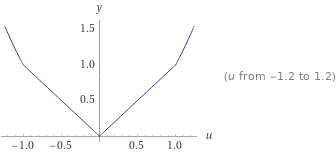
\includegraphics[scale=1.1]{function_u.png}
\caption{The piecewise defined lower semi-continuous function $I(u)$. The slope of $I(u)$ is $\pm 1$ when $|u|\leq 1$ and $\pm 2$ when $|u|> 1$. }
\end{center}
\end{figure}
By construction, $I$ is smooth away from $u=0$ and $u=\pm 1$, so the subdifferential is the derivative $I'(u)$. At $u=0$, lines with slopes of $1$ and $-1$ lie below the graph of $I$. At $u=1$, lines with slopes between $1$ and $2$ lie below the graph of $I$. Also, at $u=-1$, lines with slopes between $-2$ and $-1$ lie below the graph of $I$. Therefore
$$\partial I(u):=
  \begin{cases} 
      \{2u\} & \text{if $u< -1$} \\
      [-2,-1] & \text{if $u=-1$} \\
      \{-1\} & \text{if $-1<u<0$} \\
      [-1,1] & \text{if $u=0$} \\
      \{1\} & \text{if $0 < u < 1$} \\
      [1,2] & \text{if $u=1$} \\
      \{2u\} & \text{if $u > 1$}.
   \end{cases}
$$
By the theory of gradient flows in Evans, we know that the gradient flow
$$
  \begin{cases} 
      u'\in -\partial I[u]\quad (t>0)\\
      u(0)=u_0
   \end{cases}
$$
has a unique continuous solution $u(t)=S(t)u_0$. We investigate the solution when $u_0>1$.

When $u>1$, $\partial I[u]=\{2u\}$, so we have that $u'=-2u$ and therefore $u(t)=u_0e^{-2t}$. This is true until $u(t)$ reaches $u=1$, which happens when $1 = u_0e^{-2t}$ or $t= (1/2)\ln(u_0).$ We now move to $u\in (0,1)$. Here, $u'=-1$ and therefore $u(t)=-t+u_1.$ At $u=1$, we have that $1=-t+u_1=-(1/2)\ln(u_0)$ so that $u_1 = 1+(1/2)\ln(u_0)$. Hence $u(t)=1-(t-(1/2)\ln(u_0))$. This is true until $u(t)$ reaches $0$, where $t=1+(1/2)\ln(u_0)$. For $u \leq 0$, we have that $u(t)\equiv \text{constant}$ by construction. Combining all of these cases
$$u(t)=
  \begin{cases} 
      u_0e^{-2t} & \text{if $0\leq t \leq (1/2)\ln(u_0)$}\\
      1-(t-(1/2)\ln(u_0) & \text{if $(1/2)\ln(u_0) \leq t \leq (1/2)\ln(u_0) + 1$}\\
      0 & \text{if $t\geq (1/2)\ln(u_0) + 1$}.
   \end{cases}
$$
Therefore we can choose two initial conditions $u_0$ and $\hat{u}_0$ and then go forward in time $t$. Eventually there will be a time $t>0$ such that $S(t)u_0=S(t)\hat{u}_0=0$. Thus, the flow is irreversible.


\end{proof}
\phantomsection
\subsection{\textbf{9.7.12}} Let $u=u(x,t)$ denote the height at $x\in\mathbb R^2$ of a sandpile that grows as sand is added at a rate $f=f(x,t)\geq 0$. We assume the stability condition
$$|Du|\leq 1,$$
meaning that nowhere can the sandpile have slope greater than $1$. As usual, $D_xu=Du$. We propose the dynamics
$$u_t - \operatorname{div}(ADu)=f\quad\text{in $\mathbb R^2 \times (0,\infty)$},$$
where $a=a(x,t)\geq 0$ describes the flow rate of sand rolling downhill, that is, in the direction $-Du$. Suppose that 
$$\operatorname{spt}a \subseteq \{|Du|=1\},$$
so that the sand flows downhill only if the slope is one.

Show that the foregoing implies
$$f-u_t\in \partial I[u],$$
for the convex function
$$I(u):=
  \begin{cases} 
      0 & \text{if $u\in L^2(\mathbb R^2),~ |Du|\leq 1~a.e.$} \\
      \infty & \text{otherwise}.
   \end{cases}
$$
\begin{proof}
We follow the analysis done by Aronsson, Evans, and Wu in \cite{ARONSSON1996304} and \cite{evans1997partial}. We first proceed informally and analyze the physical aspects of the model.

Consider the non-linear p-Laplacian
$$\Delta_p u = \operatorname{div}(|Du|^{p-2}Du)$$
which for large values of $p$ is known as a prototype of a slow/fast diffusion operator. We are interested in understanding what happens in the fast and slow diffusion regions in the limit as $p\to\infty$. This problem is related to existing techniques known for Monge–Kantorovich type optimal
mass transfer problems. We introduce some standard notation from convex analysis. First, we define
$$\mathbb K := \{u\in L^2(\mathbb R^n)~ : ~|Du| \leq 1~a.e\}$$
and
$$I(u):=
  \begin{cases} 
      0 & \text{if $u\in \mathbb K$} \\
      \infty & \text{otherwise}.
   \end{cases}
$$
Here $u^*$ minimizes $K[\cdot]$ over $\mathbb K$. Its corresponding Euler-Lagrange equation is
\begin{equation}f^+ - f^- \in I[u^*]\end{equation}
which is defined as
$$I[v] \geq I[u^*] + (f^+ - f^-, v-u^*)_{L^2}$$
for every $v\in L^2(\mathbb R^n)$. We first rewrite $(25)$ in a more familiar form.
\newline
\begin{lemma}
Suppose that $f^+$ and $f^-$ are Lipschitz continuous. 

$(i)$ Then there exists a nonnegative $L^{\infty}$ function $a$ such that
\begin{equation}-\operatorname{div}(aDu^*)=f^+ - f^- \quad \text{in $\mathbb R^n$}.\end{equation}
$(ii)$ In addition
$$|Du|=1\quad \text{a.e. on the set $\{a>0\}$.}$$
Here, $a$ is known as the transport density. The PDE $(26)$ is nonlinear and $a$ is a Lagrange multiplier corresponding to the constraint $|Du^*|\leq 1$.
\end{lemma}

Sketch of Proof: Let $n+1 \leq p < \infty$. We then approximate by the quasilinear PDE defined for the p-Laplacian
\begin{equation}-\operatorname{div}(|Du_p|^{p-2}Du_p)= f^+ - f^-,\end{equation}
which corresponds to maximizing 
$$K_p[u]:=\int_{\mathbb R^n} u\left(f^+ - f^-\right) -\frac{1}{p}|Du|^p \, dz.$$
By the maximum principle, we find that
$$\sup_p |u_p|,|Du_p|,|Du_p|^p \leq C < \infty$$
for some constant $C\in(0,\infty)$. It then follows that there exists a sequence $p_k \to \infty$ such that
$$
  \begin{cases} 
      u_{p_k} \to u^* & \text{locally uniformly} \\
      Du_{p_k} \to Du^* & \text{boundedly, a.e.} \\
      |Du_{p_k}|^{p-2} \rightharpoonup a & \text{weakly $*$ in $L^{\infty}$}.
   \end{cases}
$$
Therefore, we can pass to the limit in $(27)$ to obtain $(26)$. 

For this problem, we have a sandpile model that evolves over time. In a physical context, it is a Monge–Kantorovich mass transfer mechanism which interacts on a fast time scale. As $u$ is the height of the sandpile, we impose the constraint 
\begin{equation}|Du| \leq 1\end{equation}
everywhere. The constraint has the physical interpretation that the the slope will not remain in equilibrium and that the sand will flow downhill when the slope is one. Suppose $f\geq 0$ is a source term which represents the rate at which sand is added to the sandpile whose initial height is zero. This would initially suggest that the model would be $u_t=f$ in any region where the constraint $(28)$ is active. However, adding more sand in a particular location would break the constraint and it would be perfectly reasonable to expect that these newly added sand particles would instantaneously roll downhill. The particles would continue rolling downhill until stopping at a rest state where adding new particles maintains the constraint.

This gives the following evolutionary model for growing sandpiles
$$
  \begin{cases} 
      f-u_t = \partial I[u] & (t>0) \\
      u = 0 & (t=0),
   \end{cases}
$$
where $I[\cdot]$ is defined by
$$I[v] \geq I[u^*] + (f^+ - f^-, v-u^*)_{L^2}$$
for every $v\in L^2(\mathbb R^n)$. Applying Lemma $8$ we see that $f^+ = f$ and $f^- = u_t$ so that $u_t - \operatorname{div}(ADu)=f$. The physical interpretation is that for every moment of time, the mass $d\mu^+ = f^+(\cdot,t)dx$ is instantly and optimally transported downhill by the potential $u(\cdot,t)$ into the mass $d\mu^- = u_t(\cdot,t)dy$. Therefore, the height $u(\cdot,t)$ of the sandpile is also the potential which generates the Monge–Kantorovich reallocation of $f^+dx $ to $u_tdy$. This relation forces the dynamics of the growing sandpile model. 

Now, we analyze why the dynamics give the evolution equation. Let us consider evolutions governed by the p-Laplacian:
$$\begin{cases} 
      u_{p,t} - \Delta_p u_p = f_p & \text{in $\mathbb R^n \times (0,\infty)$}\\
      u_p = g & \text{on $\mathbb R^n \times \{t=0\}$}
   \end{cases}$$
and study the behavior of the solutions $u_p$ as $p\to\infty$. Here $f\geq 0$ represents
a given source term, which we interpret physically as adding material to an
evolving system. As $p\to\infty$, we will see that $u_p\to p$ and that the limit $u$ solves the evolution equation
$$f-u_t = \partial I[u], \quad t>0.$$
We start by sending $p\to\infty$. Then for every $T>0$ we have that the functions $\{u_p\}_{p\geq n+1}$ are bounded in $L^{\infty}(\mathbb R^n \times [0,T])$ and $\{Du_p,u_{p,t}\}_{p\geq n+1}$ are bounded in $L^2(\mathbb R^n \times [0,T])$.
Further, the functions $\{u_p\}_{p\geq n+1}$ have a uniform bound supported in $\mathbb R^n \times [0,T]$. Therefore we can extract a sequence $p_i \to \infty$ and a limit $u$ so that for every $T>0$
\begin{equation}
  \begin{cases} 
      u_{p_i} \to u & \text{a.e. and in $L^2\left(\mathbb R^n \times (0,T)\right)$}\\
      Du_{p_i} \rightharpoonup Du, ~ u_{p_{i,t}} \rightharpoonup u_t & \text{weakly in $L^2\left(\mathbb R^n \times (0,T)\right)$}.
   \end{cases}
\end{equation}
We then reinterpret the evolution PDE as
$$f_p - u_{p,t}=\partial I_p[u_p], \quad t>0, $$
where we will send $p\to\infty$ to recover the original PDE. We make some explicit assumptions regarding the source terms $\{f_p\}_{p\geq n+1}.$ For this, we select $m$ distinct points $\{d_k\}_{k=1}^m \subset \mathbb R^n$ and $m$ smooth, nonnegative functions of time $\{f_k(t)\}_{k=1}^m$. This will imply that the measure
$$f=\sum_{k=1}^m f_k(t)\delta_{d_k}(x)$$
will record point sources at the sites $\{d_k\}_{k=1}^m$ with rates $\{f_k(t)\}_{k=1}^m$. For every $k=1,\ldots,m$ and $n+1\leq p \leq \infty$ we let $d_p^k:\mathbb R^n \to \mathbb R$ be smooth functions satisfying
 $$\begin{cases} 
      \operatorname{supp}(d_k^p)\subset B(d_k,r_p), & d_k^p\geq 0,\\
      \int_{B(d_k,r_p)} d_k^p \,dx =1 & \text{as $p\to\infty$}
   \end{cases}$$
 where $r_p \to 0$ as $p\to\infty$. This is why we require $\operatorname{spt}a \subseteq \{|Du|=1\}.$ We then take
 $$f_p(x,t)=\sum_{k=1}^m f_k(t) d_k^p(x)\quad (n+1\leq p \leq \infty)$$
 as a smooth approximation to $f$. With this setup, we arrive at the following 

\begin{theorem}
The limit function $u$ defined by $(29)$ satisfies $$f-u_t \in \partial I[u] \quad \text{a.e. $t>0$.}$$
\end{theorem}
Setup of Theorem $9$: We interpret $f-u_t \in \partial I[u] $ as
\begin{equation}I[v] \geq I[u] + \int_{\mathbb R^n} (f(x,t) - u_t(x,t))(v-u(x,t))\,dx,\end{equation}
for every $v\in \L^2(\mathbb R^n)$ at a.e. $t>0$. We also suppose that $v$ is Lipschitz and that the Lipschitz constant is at most one. Then the expression 
$$\int_{\mathbb R^n} f(x,t)(v - u(x,t))\,dx$$
may defined as
$$\sum_{k=1}^m f_k(t)(v(d_k)-u(d_k,t)).$$

Proof of Theorem $9$: As $|Du|\leq 1$, we have that $I\left[u(\cdot,t)\right]=0$ for a.e. $t>0$. We will also assume that $v$ has compact support. To verify $(30)$ is true, we need to show that
\begin{equation}
\int_{\mathbb R^n} (f(x,t) - u_t(x,t))(v-u(x,t))\,dx \leq 0
\end{equation}
for a.e. $t>0$. To do this, we fix two times $0 < t_1 < t_2$. Our original PDE becomes
$$f_p-u_{p,t} = \partial I_p[u_p].$$
This implies
\begin{align}
(t_2-t_1)I_p[v] &\geq \int_{t_1}^{t_2} I\left[u_p(\cdot,t)\right]\,dt + \int_{t_1}^{t_2} \int_{\mathbb R^n} (f_p(x,t) - u_{p,t}(x,t))(v-u_p(x,t))\,dxdt \nonumber\\& \geq
\int_{t_1}^{t_2} \int_{\mathbb R^n} (f_p(x,t) - u_{p.t}(x,t))(v-u_p(x,t))\,dxdt, 
\end{align}
Then since $|Dv|\leq 1$ a.e. and $v$ is compactly supported, we have
$$\lim_{p\to\infty}I_p[v]=0.$$
By $(29)$, we see that the weak convergence implies
\begin{equation}\int_{t_1}^{t_2} \int_{\mathbb R^n} u_{p_{i,t}}(x,t) (v - u_{p_i}(x,t))\,dxdt \to \int_{t_1}^{t_2} \int_{\mathbb R^n} u_t(x,t)(v-u(x,t))\,dxdt.
\end{equation}
It remains to show that
\begin{equation}
\int_{t_1}^{t_2}\int_{\mathbb R^n} f_{p_i}(x,t)(v - u_{p_i}(x,t))\,dxdt \to \sum_{k=1}^m \int_{t_1}^{t_2} f_k(t)(v(d_k)-u(d_k,t))\,dt.
\end{equation}
Since $\operatorname{spt}(a)\subseteq \{|Du|=1\}$ it follows that $\operatorname{spt}(d_k^p)\subseteq \{|Du|=1\}$ which implies
\begin{equation}\int_{t_1}^{t_2}\int_{\mathbb R^n} f_{p_i}(x,t)v\,dxdt\to \int_{t_1}^{t_2} \sum_{k=1}^m f_k(t) v(d_k)\,dt.
\end{equation}
So for a.e. $t > 0$ and $p\geq 2n$ we obtain
$$\norm{u_p(\cdot,t)}_{C^{0,1/2}} \leq C\left(\norm{Du_p(\cdot,t)}_{L^{2n}}+\norm{u_p(\cdot,t)}_{L^{\infty}}\right).$$
The $C^{0,1/2}$ norm is defined by
$$\norm{w}_{C^{0,1/2}}=\norm{w}_{L^{\infty}}+\sup_{x\neq y}\frac{|w(x)-w(y)|}{|x-y|^{1/2}
}.$$
This gives
\begin{align*}
    \int_{t_1}^{t_2} \norm{u_p(x,t)}_{C^{0,1/2}}\,dt &\leq
    C + C\int_{t_1}^{t_2}\norm{Du_p(x,t)}_{L^{2n}}\,dt\\&=
    C + C\left(\int_{t_1}^{t_2}\int_{\mathbb R^n}|Du_p(x,t)|^{2n}\,dxdt\right)^{1/2n}\\&\leq
    C + C\left(\int_{t_1}^{t_2}\int_{\mathbb R^n}|Du_p(x,t)|^{p}\,dxdt\right)^{1/p}\\&\leq C,
\end{align*}
where all of the integrations are done over finite values. Therefore we find
\begin{align*}
\int_{t_1}^{t_2} \int_{\mathbb R^n} f_{p_i}(x,t)u_{p_i}(x,t)\,dxdt&=\sum_{k=1}^m \int_{t_1}^{t_2} f_k(t) \int_{B(d_k, r_{p_i})} d_k^{p_i}(x)u_{p_i}(x,t)\,dxdt\\&=
\sum_{k=1}^m \int_{t_1}^{t_2} f_k(t)u_{p_i}(d_k,t)\,dt + \\&
\sum_{k=1}^m \int_{t_1}^{t_2} f_k(t) \int_{B(d_k, r_{p_i})}d_k^{p_i}(x)\Big(u_{p_i}(x,t) - u_{p_i}(d_k,t)\Big)\,dxdt \\&:= A_1 + A_2.
\end{align*}
We bound both of these expressions. First
\begin{align*}
|A_2| &\leq C \sum_{k=1}^m \int_{t_1}^{t_2}\sup_{B(d_k,r_{p_i})}|u_{p_i}(x,t)- u_{p_i}(d_k,t)|\,dt \\ &\leq
Cr_{p_i}^{1/2}\int_{t_1}^{t_2}\norm{u_{p_i}(x,t)}_{C^{0,1/2}}\,dt\\&\leq
Cr_{p_i}^{1/2},
\end{align*}
because  $\int_{t_1}^{t_2} \norm{u_p(x,t)}_{C^{0,1/2}}\,dt\leq C$. We then fix $r>0$ to find
\begin{align*}
    A_1 &= \sum_{k=1}^m \int_{t_1}^{t_2} f_k(t)u_{p_i}(d_k,t)\,dt\\&=
    \sum_{k=1}^m \int_{t_1}^{t_2} f_k(t) \dashint_{B(d_k,r)}u_{p_i}(d_k,t)-u_{p_i}(x,t)\,dxdt\\&+
    \sum_{k=1}^m \int_{t_1}^{t_2} f_k(t) \dashint_{B(d_k,r)}u_{p_i}(x,t)\,dxdt \\&:= B_1+B_2.
\end{align*}
Proceeding as before,
$$|B_1|\leq Cr^{1/2}.$$
To estimate $B_2$ we apply $(29)$ and pass to limits to find
\begin{align*}\limsup_{p_i\to\infty}&\left|\int_{t_1}^{t_2}\int_{\mathbb R^n} f_{p_i}(x,t)u_{p_i}(x,t)\,dxdt - \sum_{k=1}^m\int_{t_1}^{t_2} f_k(t) \dashint_{B(d_k,r)}u(x,t)\,dxdt\right|
\\&\leq Cr^{1/2}.
\end{align*}
Now since $|Du|\leq 1$ a.e. we have
$$\sum_{k=1}^m \dashint_{B(d_k,r)}|u(x,t)-u(d_k,t)|\,dx \leq Cr,$$
which implies
$$\limsup_{p_i\to\infty}\left|\int_{t_1}^{t_2}\int_{\mathbb R^n} f_{p_i}(x,t)u_{p_i}(x,t)\,dxdt - \sum_{k=1}^m\int_{t_1}^{t_2} f_k(t)u(d_k,t)\,dt\right|\leq Cr^{1/2}$$
for every $r>0$. In combination with $(35)$, this justifies $(34)$. 

Then $(32)-(34)$ imply
$$0 \geq \int_{t_1}^{t_2} \sum_{k=1}^m f_k(t) (v(d_k)-u(d_k,t))\,dt -\int_{t_1}^{t_2}\int_{\mathbb R^n} u_t(x,t) (v-u(x,t))\,dxdt$$
for every $0\leq t_1 < t_2$ and $v$ as above. Hence
$$0 \geq \sum_{k=1}^m f_k(t) (v(d_k)-u(d_k,t)) -\int_{\mathbb R^n} u_t(x,t) (v-u(x,t))\,dx$$
for a.e. $t\geq 0$ and $v$. This establishes $(31)$ and completes the proof. The exercise then follows from the assumptions of $|Du|\leq 1$ and $\operatorname{spt}a \subseteq \{|Du|=1\}$ which are included in the assumptions of Theorem $9$. The last assumption that 
$$u_t - \operatorname{div(Adu)}=f \quad \text{in  $\mathbb R^2 \times (0,\infty)$},$$
is used in defining the degenerate parabolic PDE
$$\begin{cases}
u_{p,t} - \operatorname{div}(|Du_p|^{p-2}Du_p)=f_p &\text{in $\mathbb R^n \times (0,\infty)$} \\
u_p = g & \text{on $\mathbb R^n \times \{t=0\}$}
\end{cases}$$
where $n+1\leq p < \infty$ taking the limit as $p\to\infty$ gives the desired evolution equation.
\end{proof}
\phantomsection
\subsection{\textbf{9.7.13}} Assume $u$ is a smooth solution of the gradient flow system $(33)$ in $\S 9.6.3$, where $L$ satisfies the uniform convexity condition $(29)$. Show there exists constants $C,\gamma > 0$ such that
$$\int_U u^2_t(x,t) \,dx \leq Ce^{-\gamma t}\quad (t>0).$$
\begin{proof}

The idea behind this problem is that convex gradient flows converge exponentially to a minimizer.

We first review the theory of gradient flows. In general, a partial differential equation is a gradient flow of an energy functional
$E : X\to (-\infty,+\infty]$ on a metric space $(X,d)$ if the equation may be written as
$$\frac{d}{dt} u(t)= -\nabla_d E(u(t)), \quad u(0)=u\in X,$$
for a generalized notion of gradient $\nabla_d.$
\newline
\\
To get a feel for gradient flows in $L^2(U)$, we review the heat equation. It is defined by the Dirichlet energy
$$ E(u):=
  \begin{cases} 
      \frac{1}{2}\int_U |\nabla u(x)|^2\,dx, & \text{for $u\in H_0^1(U)$}\\
      +\infty & \text{otherwise}.
   \end{cases}
$$
Here $E(u)$ isn't continuous with respect to the $L^2(U)$ norm, even on the restricted set $\mathcal{G}:=H_0^1(U)\cap H^2(U)$. However, its directional derivatives are well defined for every $u\in\mathcal{G}$ since
$$\lim_{h\to 0} \frac{E(u+hv) - E(u)}{h}=\int_U \nabla u \cdot \nabla v = -\int_U \Delta u v, \quad \forall v\in C_c^{\infty}(U).$$
By this, we define $\nabla_{L^2} E(u)$ to be the vector field satisfying 
$$(\nabla_{L^2}  E(u), v)_{L^2(U)}=\lim_{h\to 0} \frac{E(u+hv) - E(u)}{h}=(-\Delta u, v)_{L^2(U)},\quad \forall v\in L^2(U).$$
Hence, the gradient flow of the Dirichlet energy is the heat equation
$$\frac{d}{dt}u(t) = -\nabla_{L^2}  E(u(t))=\Delta u(t).$$
By linearity of the gradient and convexity of $|\cdot|^2$, the Dirichlet energy is convex on $L^2(U).$

We now review gradient flows on Hilbert spaces. In general, the theory can be seen as a nonlinear, infinite dimensional
generalization of the theory of ordinary differential equations. Suppose we have a functional $E:\mathcal{H}\to \mathbb R \cup \{+\infty\}$ on a Hilbert space $\mathcal{H}$. We then define the Hilbert space gradient analogously to the definition of $\nabla_{L^2}$. We also define three other properties. 

\textbf{Definition 1} (Hilbert space gradient). $\nabla_\mathcal{H} E(u)\in\mathcal{H}$ is a Hilbert space gradient of $E$ at $u$ if
$$(\nabla_\mathcal{H} E(u),v) = \lim_{h\to 0} \frac{E(u+hv) - E(u)}{h}, \quad \forall v\in\mathcal{H}.$$
\textbf{Definition 2} ($L^2$ gradient and functional derivative). Consider the class of integral functions $E(u)=\int F(x,u(x),\nabla u(x))dx$ on $L^2(U)$. If $u$ is sufficiently regular then the functional derivative $\frac{\delta E}{\delta u}\in L^2(U)$ exists and satisfies 
$$\lim_{h\to 0} \frac{E(u+hv) - E(u)}{h} =
\int_U \frac{\delta E}{\delta u}v, \quad \forall v\in C_c^{\infty}(U).$$
In our case, we identify $\nabla_{L^2} E(u)$ with $\frac{\delta E}{\delta u}$. With this definition of Hilbert space gradient, we define the Hilbert space gradient flow.

\textbf{Definition 3} (Hilbert space gradient flow). The gradient flow of $E$ with respect to $\mathcal{H}$ is
$$\frac{d}{dt}u(t)=-\nabla_\mathcal{H}E(u(t)), \quad u(0)=u.$$

\textbf{Definition 4} (Convexity inequality). Given $\theta\in\mathbb R$ and a functional $E:\mathcal{H} \to \mathbb R \cup \{+\infty\}$ we obtain for convex $E$
$$(\nabla E(u) - \nabla E(v), v - u)\geq \frac{\theta}{2}|v - u |^2.$$
These give rise to the exponential decay of the gradient. That is, 
\begin{equation}|\nabla E(u(t))|\leq e^{-\theta t}|\nabla E(u(0))|.\end{equation}
To see this, we impose the additional assumption that for all $u\in\mathcal{G}:=H_0^1(U)\cap H^2(U)$, there exists $D^2 E(u):\mathcal{G}\to\mathcal{H}$ satisfying 
$$(D^2 E(u)v,w)=\lim_{h\to 0}\frac{(\nabla E(u+hv)-\nabla E(u),w)}{h},\quad \forall v\in\mathcal{G}.$$
The convexity inequality then implies
$$(D^2 E(u)v,v)=\lim_{h\to 0}\frac{(\nabla E(u+hv)-\nabla E(u),hv)}{h^2}\geq
\lim_{h\to 0}\frac{\theta}{2}\frac{|hv|^2}{h^2}=\frac{\theta}{2}|v|^2.
$$
Therefore
$$\frac{d}{dt}\frac{1}{2}|\nabla E(u(t))|^2=-(D^2E(u(t))\nabla E(u(t)),\nabla E(u(t)))\leq -\frac{\theta}{2}|\nabla E(u(t))|^2,$$
and integrating yields the inequality $(15)$. In our case
$$u_t = -\nabla E(u(t))$$
so by defining $H(t):=|\nabla E(u(t))|^2$ we have 
$$\frac{d}{dt}\frac{1}{2}H(t) \leq - \frac{\theta}{2} H(t).$$
By the inequality 
$$\frac{d}{dt}\left(H(t)e^{-\theta t}\right) = H'(t)e^{-\theta t} - \theta H(t) e^{-\theta t} \leq 0$$
we see that $H(t) \leq H(0)e^{-\theta t}$ therefore implying
$$\int_U u_t^2(x,t)\,dx \leq e^{-\theta t}\int_U |\nabla E(u(0))|^2 = Ce^{-\gamma t}.$$
The same analysis follows from applying Gronwall's inequality after integration.

Remark: Perhaps Evans intended to ``take a more direct route to arrive at this inequality." Returning back to the energy functional
$E:L^2(U)\to\mathbb R\cup\{+\infty\}$ defined by  
$$ E(u):=
  \begin{cases} 
      \frac{1}{2}\int_U |\nabla u(x)|^2\,dx, & \text{for $u\in H_0^1(U)$}\\
      +\infty & \text{otherwise}.
   \end{cases}
$$
We integrate by parts to find 
$$\frac{d}{dt}E(u(t))=\int_U \nabla u(t)\cdot \nabla u_t(t)=-\int_U |\Delta u(t)|^2=-\norm{\nabla E(u)}_{L^2(U)}^2.$$
We may also observe that
\begin{align*}\frac{d}{dt}\norm{\nabla E(u)}_{L^2(U)}^2&=2\int_U \Delta u(t) \Delta u_t(t) \\&=
2\int_U \Delta u(t) \Delta(\Delta u(t))\\&=
-2\int_U |\nabla(\Delta u(t))|^2 \\&\leq 0,
\end{align*}
which shows that there is exponential convergence to the unique minimum of $E(u)$ over $L^2(u)$. Applying similar analysis as above with the uniform convexity condition gives
$$\frac{d}{dt}H(t) \leq - \theta H(t).$$
where $H(t)$ is the $L^2$ norm squared of the energy. Proceeding as before, we see that 
$$\frac{d}{dt}\left(H(t)e^{-\theta t}\right) = H'(t)e^{-\theta t} - \theta H(t) e^{-\theta t} \leq 0$$
implies $H(t) \leq H(0)e^{-\theta t}$. Hence
$$\int_U u_t^2(x,t)\,dx \leq e^{-\theta t}\int_U |\nabla E(u(0))|^2 = Ce^{-\gamma t}.$$




\end{proof}

\end{flushleft}
\printbibliography

\end{document}
